%%%%%%%%%%%%%%%%%%%%%%%%%%%%%%%%%%%%%%%%%%%%%%%%%%%%%%%%%%%%%%%%%%%%%%%%%%%%%%%%
%
%   Semester project, fall term 2014
%   Author: Jakob Ehrl, born 01/24/91
%   Study program: Computer science, MA 1
%   
%   Professor Dr. Francesco Mondada
%   Assistant: Dr. Stefan Witwicki
%
%%%%%%%%%%%%%%%%%%%%%%%%%%%%%%%%%%%%%%%%%%%%%%%%%%%%%%%%%%%%%%%%%%%%%%%%%%%%%%%%%

\chapter{The Robot}
%(short introduction w/ pics of the robot.)
Since the beginning we aimed to develop a robot that could move in every part of the arena and theoretically capable of grasping all the bottles.
Therefore to accomplish this goal all the strategies that have been evaluated at the beginning aimed to conceive a robot whose first characteristic was robustness. All the solutions that could be specific just to a particular situation or environment have been discarded.
Keeping in mind this idea the robot’s characteristics came up as a consequence.
Indeed the first consequence was the actual size of the robot. The width had to respect the constraint to be smaller than 45 cm in order to be able to take the ramp and access to the zone 4 of the arena.
Furthermore the robot shall not have components distant from the ground less than a certain threshold, that has been decided to be of 4 cm, so that any possible contact of these components with the rocks while passing from the zone 1 to the zone 3 would be avoided.
However, in order to be able to collect bottles, a sort of elevator was designed. The elevator didn\textsc{\char13} t respect such a constraint, while picking up bottles, but when crossing the rocky passage it could be lifted up.
Our wish was to design a small robot in order to be agile enough to easily avoid the unmodeled  obstacles represented by the bricks distributed all over the arena.
A smaller robot is more likely to avoid them with ease if compared to a bigger one that needs more precision in the maneuvers in order to accomplish the same goal.


\begin{figure}[H]
 \centering
 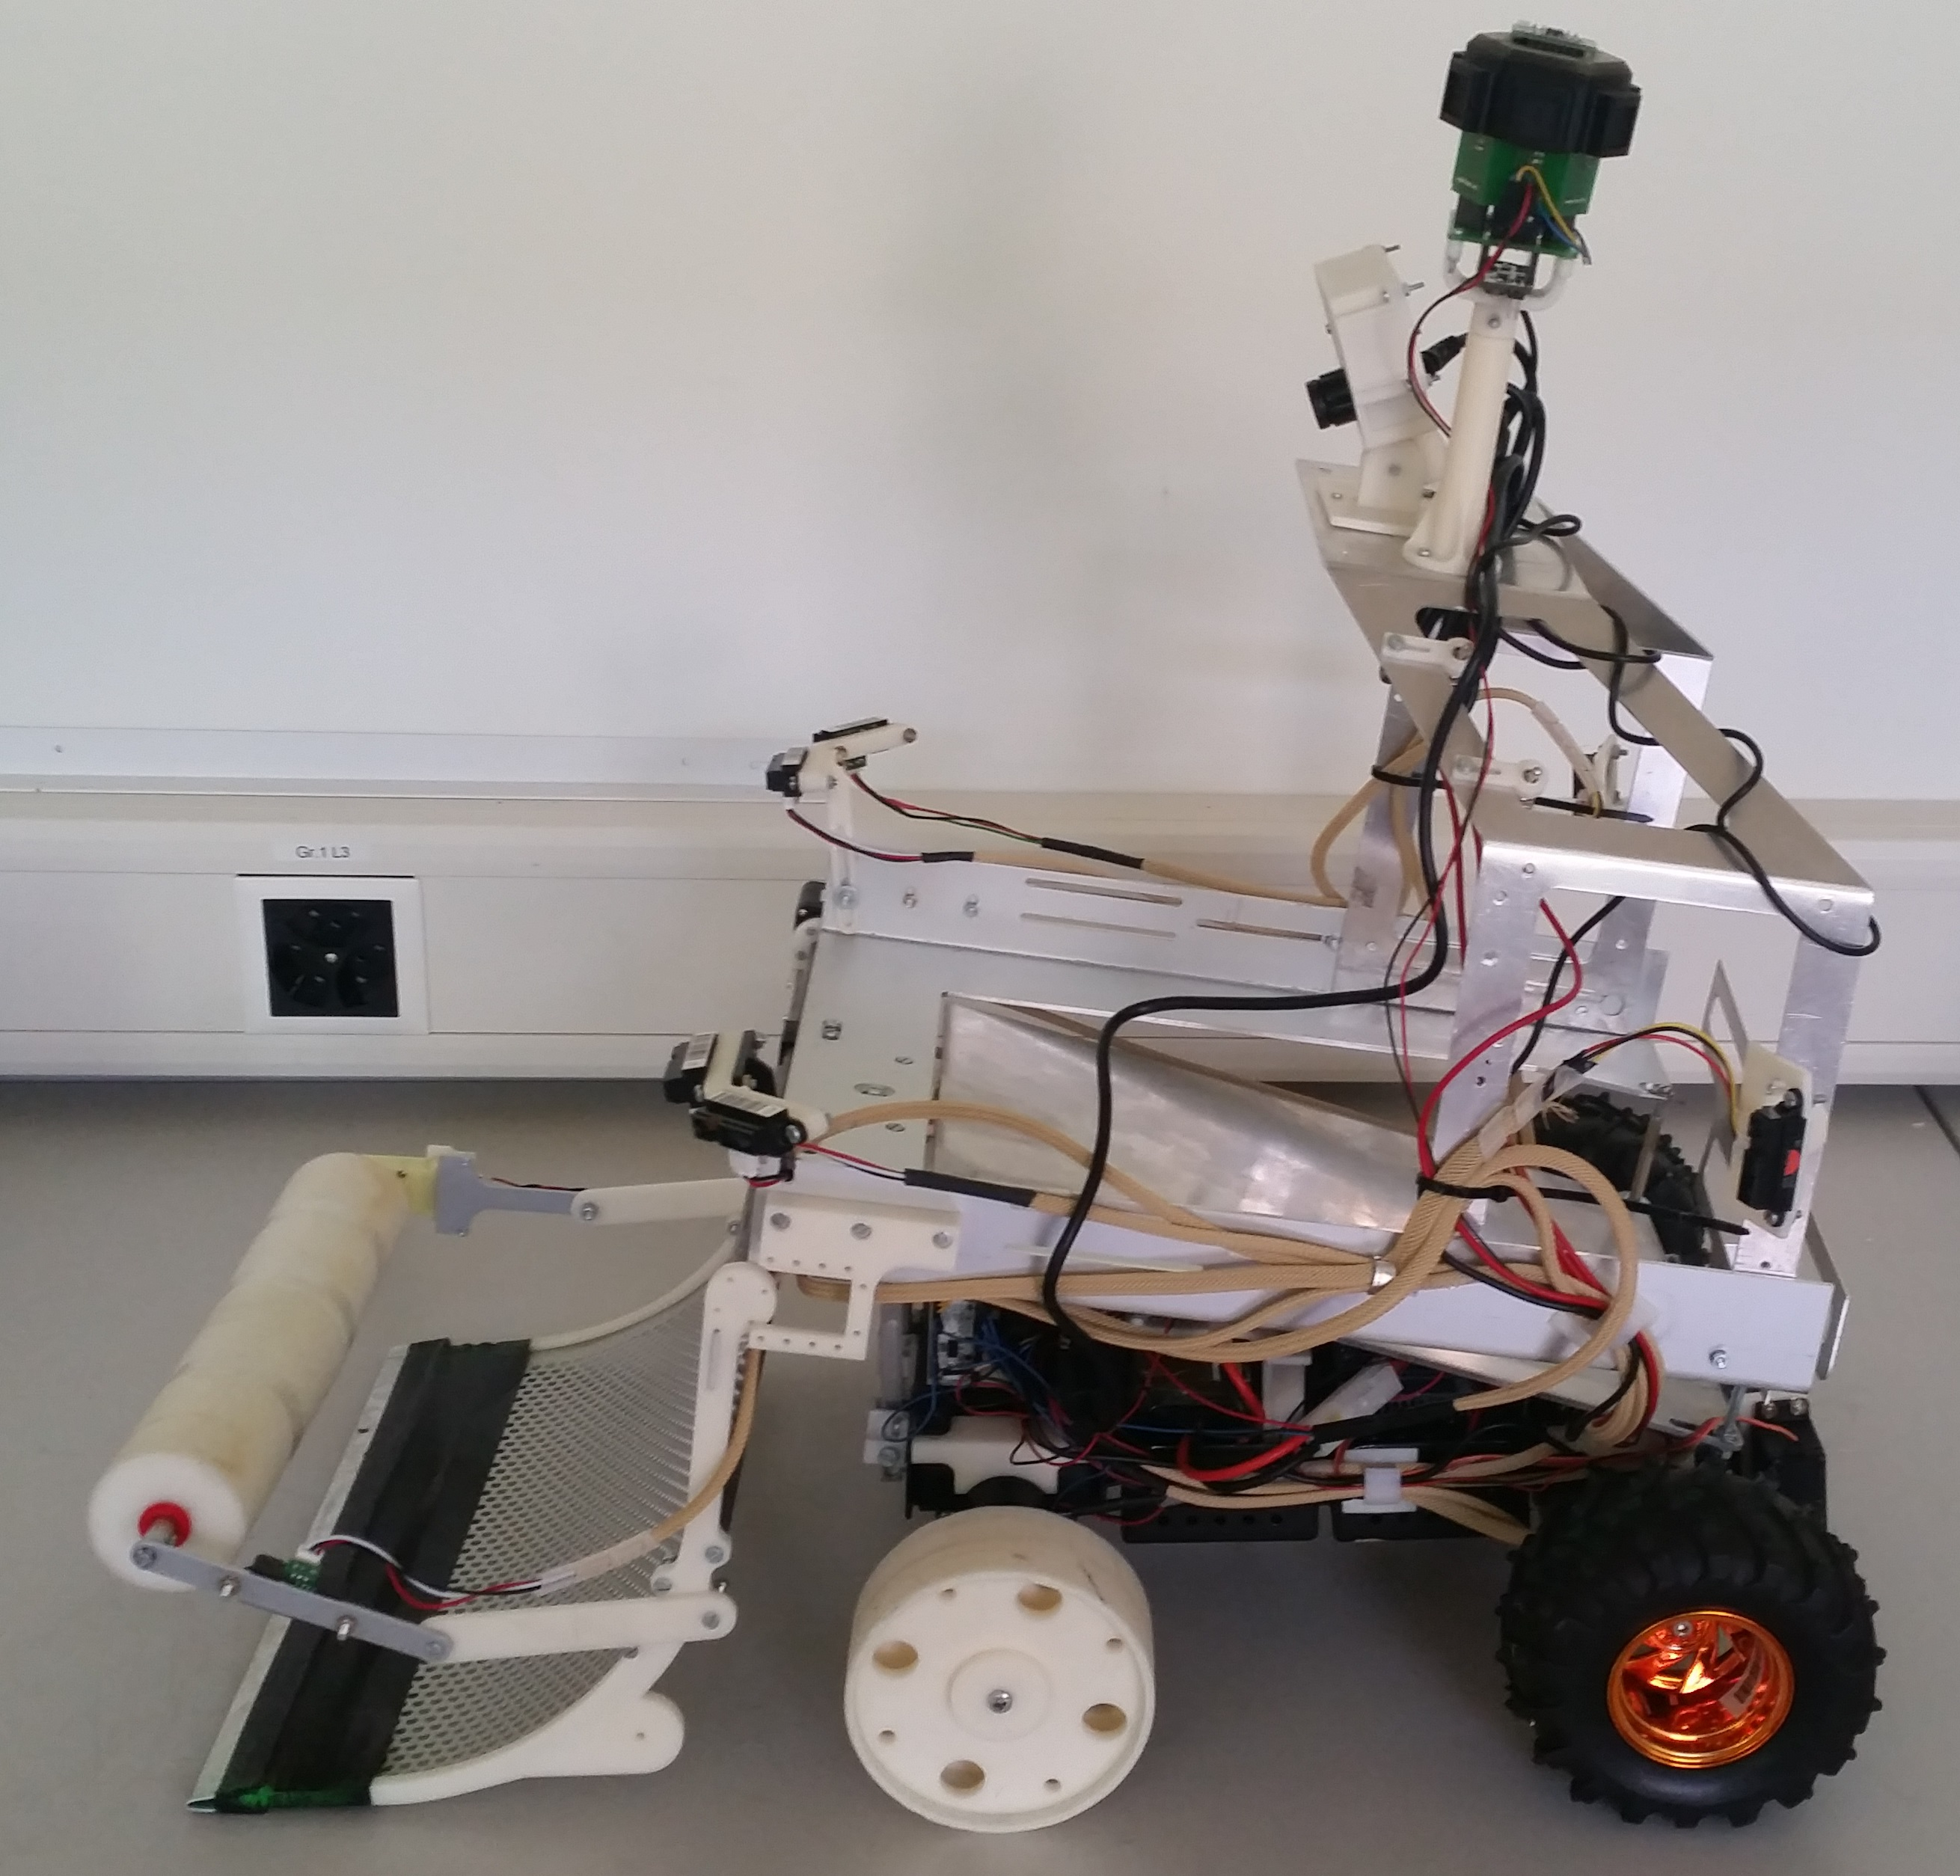
\includegraphics[width=0.8\textwidth]{robot.JPG}
 \caption{The final robot.}
\label{fig:robot}
\end{figure}

\section{Features}
The interactions of such a system with the environment are done by exploiting sensors and actuators. 
\begin{figure}[H]
\centering
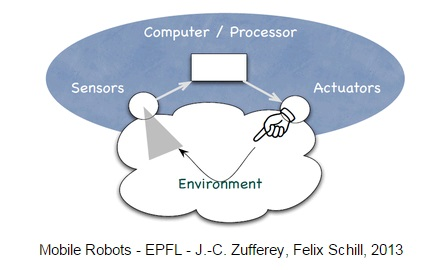
\includegraphics[width=0.8\textwidth]{RoboticSystem.jpg}
\caption{Conceptual schema of a robotic system and its interactions with the environment.}
\label{fig:RoboticSystem}
\end{figure}

As a result the main components of our robot can be clustered according to this division:
\begin{itemize}
\item Sensors
\subitem - Ultrasonic
\subitem  - IR
\subitem  - Camera
\item Brain
\subitem  - Odroid (\textit{see chapter on central processing})
\subitem  - Wild Thumper controller (\textit{see chapter on actuation})
\subitem  - 2 Arduino Micro (\textit{see chapters on localization and sensing})
\item Actuators
\subitem  - 3 Servo-Actuators
\subitem  - Brush motor
\end{itemize}

All these aspects are described in their chapters later on.\\

Using such a system the bottles will be grasped thanks to the cooperation between a rotating brush and a mobile plate (actuated by the servo) and put in a storage area above the robot in order to store  around 4 bottles before dropping them into the recycling area by opening a back door.
This storage area on the robot was conceived since we also wanted to be able to store several bottles on the robot in order to not have to return to the recycling area each time a pet bottle was grasped.
The way of grasping bottles has been thought in way to be as greedy as possible, meaning that detection of the exact position and orientation of the bottles had to be avoided because it would require a lot of time and precision from the sensors decreasing the robustness of the solution.
Therefore the way to pick up bottles resulted in a mobile plate that was feeded bottles by a rotating  sponge that could retain the bottles until the  plate reached a position from where the bottles can roll in the storage area on the robot.
The moving plate is shaped in a way that bottles don’t need to be perfectly aligned  to be grasped by the “pick-up bottle” system. Furthermore the brush can slightly move in a range of $\pm 5^{\circ}$ Avoiding the possibility of a bottle getting blocked under it.
 This characteristic has been exploited also to detect when a bottle was actually grasped. Indeed getting in the contact with a bottle, the brush had to generate more force to displace it. This change could be felt by the motor of the sponge in terms of a change in the current that could be read by the `brain of the robot'

\section{Mechanical principle}

\begin{wrapfigure}{l}{0.5\textwidth}
\begin{center}
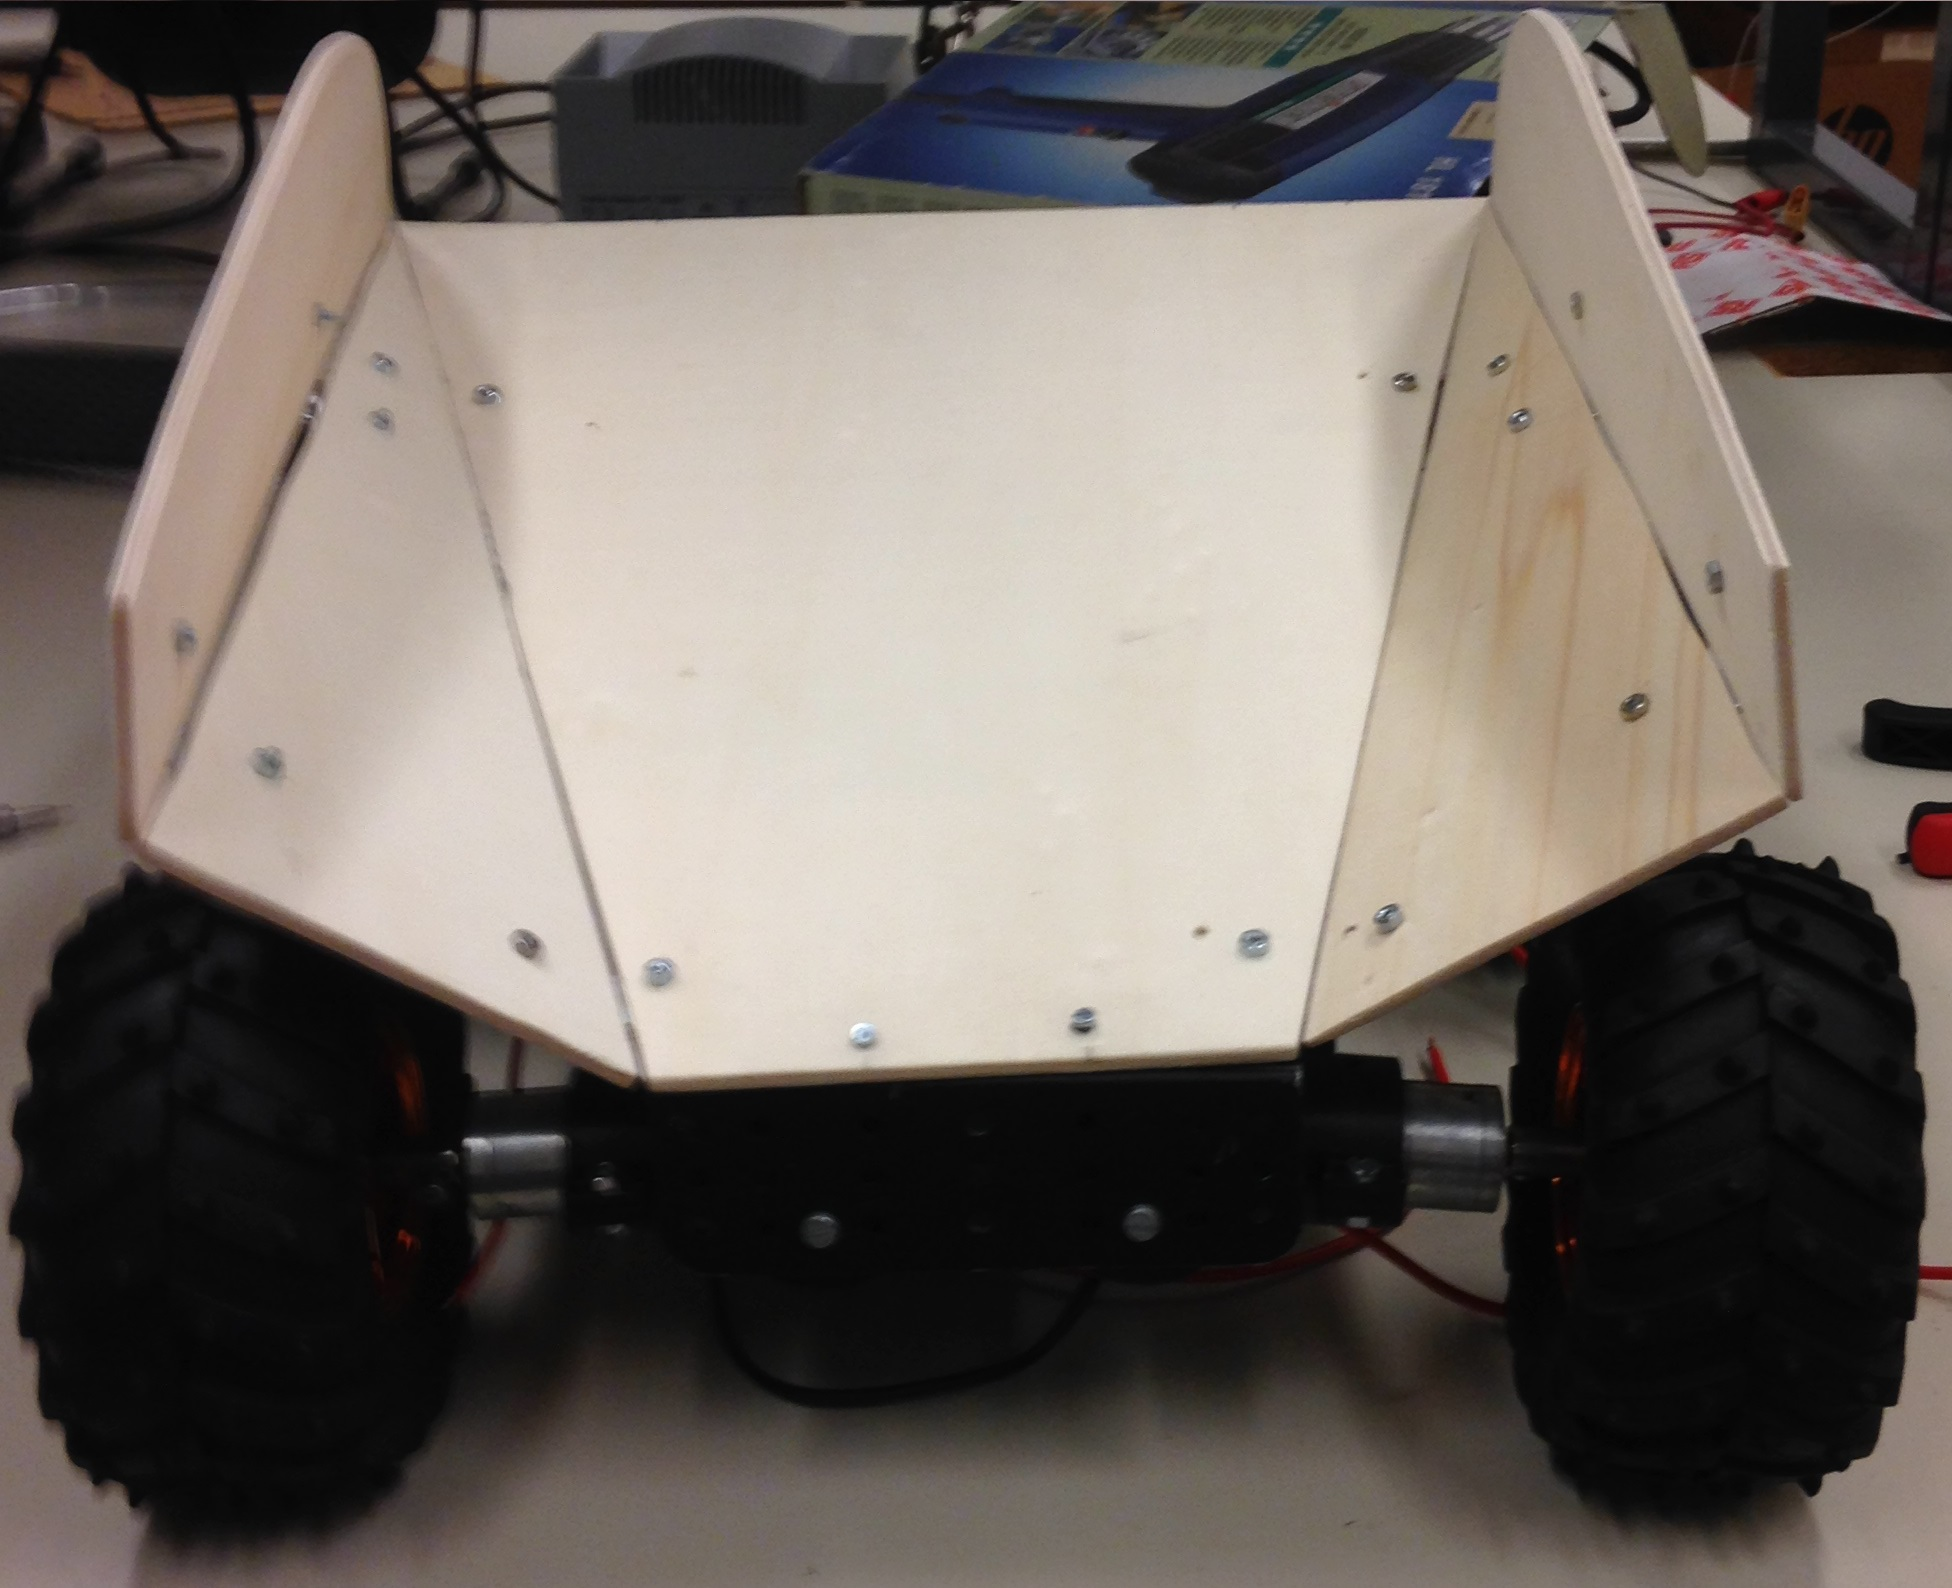
\includegraphics[width=0.3\textwidth]{WoodenModel1.JPG}
\end{center}
\caption{Back view of the robot's wooden model.}
\label{fig:WoodenModel1}
\end{wrapfigure}

After deciding the robot's working principles, in order to verify the effectiveness of our ideas, some tests of the single components constituting the robot have been conducted.
Firstly, a wooden model of the principal parts has been realized.
%Some pics of this model from different points of view are %shown in the figures below. 


During this process the experiment conducted on it allowed us to realize some small changes that have made our initial draft evolve toward the final idea.

These tests were useful to determine the effectiveness of the “pick-up bottle” system and to comprehend in which cases the bottles could get stuck in undesired positions. This made us modify the shape of the elevator removing the lateral walls that represented an obstacle for bottles not perfectly centered with respect to the center of the robot.


\begin{wrapfigure}{r}{0.5\textwidth}
\begin{center}
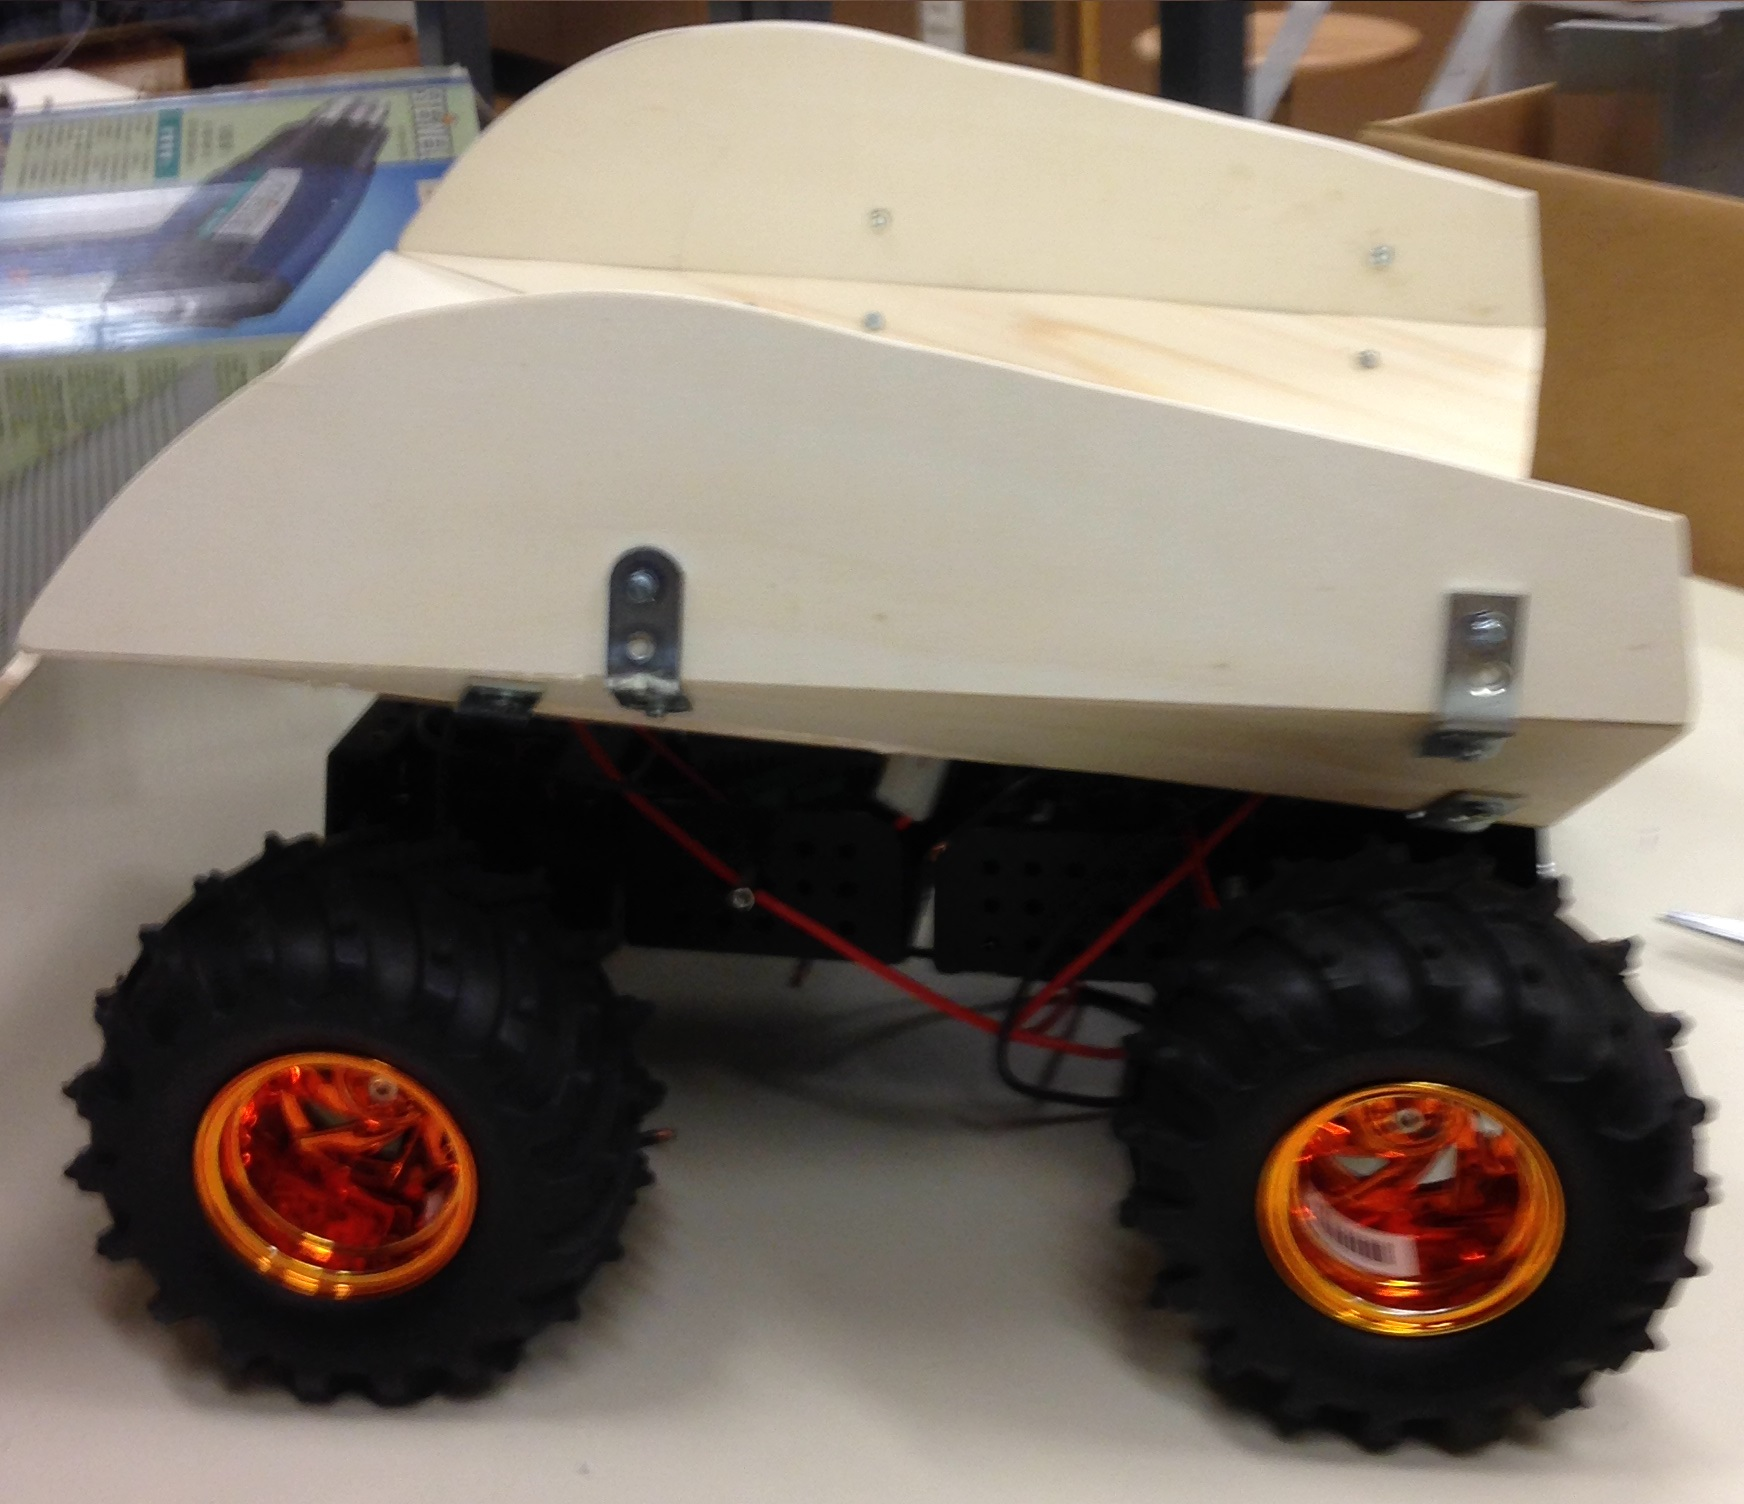
\includegraphics[width=0.3\textwidth]{WoodenModel2.JPG}
\end{center}
\caption{Lateral view of the robot's wooden model.}
\label{fig:WoodenModel2}
\end{wrapfigure}

Furthermore we shaped it in a more rounded fashion in order to allow bottles in any orientation to be successfully collected by the robot.

These modifications pointed toward the obtainment of a `greedy` mechanism that could deal with almost every possible situation, even the most challenging ones.
Furthermore, the tests on the wooden model, have made possible the optimization of the storage part in terms of:

\begin{itemize}
\item Number of bottles that could be stored
\item Space for electronics
\end{itemize}

\begin{wrapfigure}{l}{0.5\textwidth}
\begin{center}
 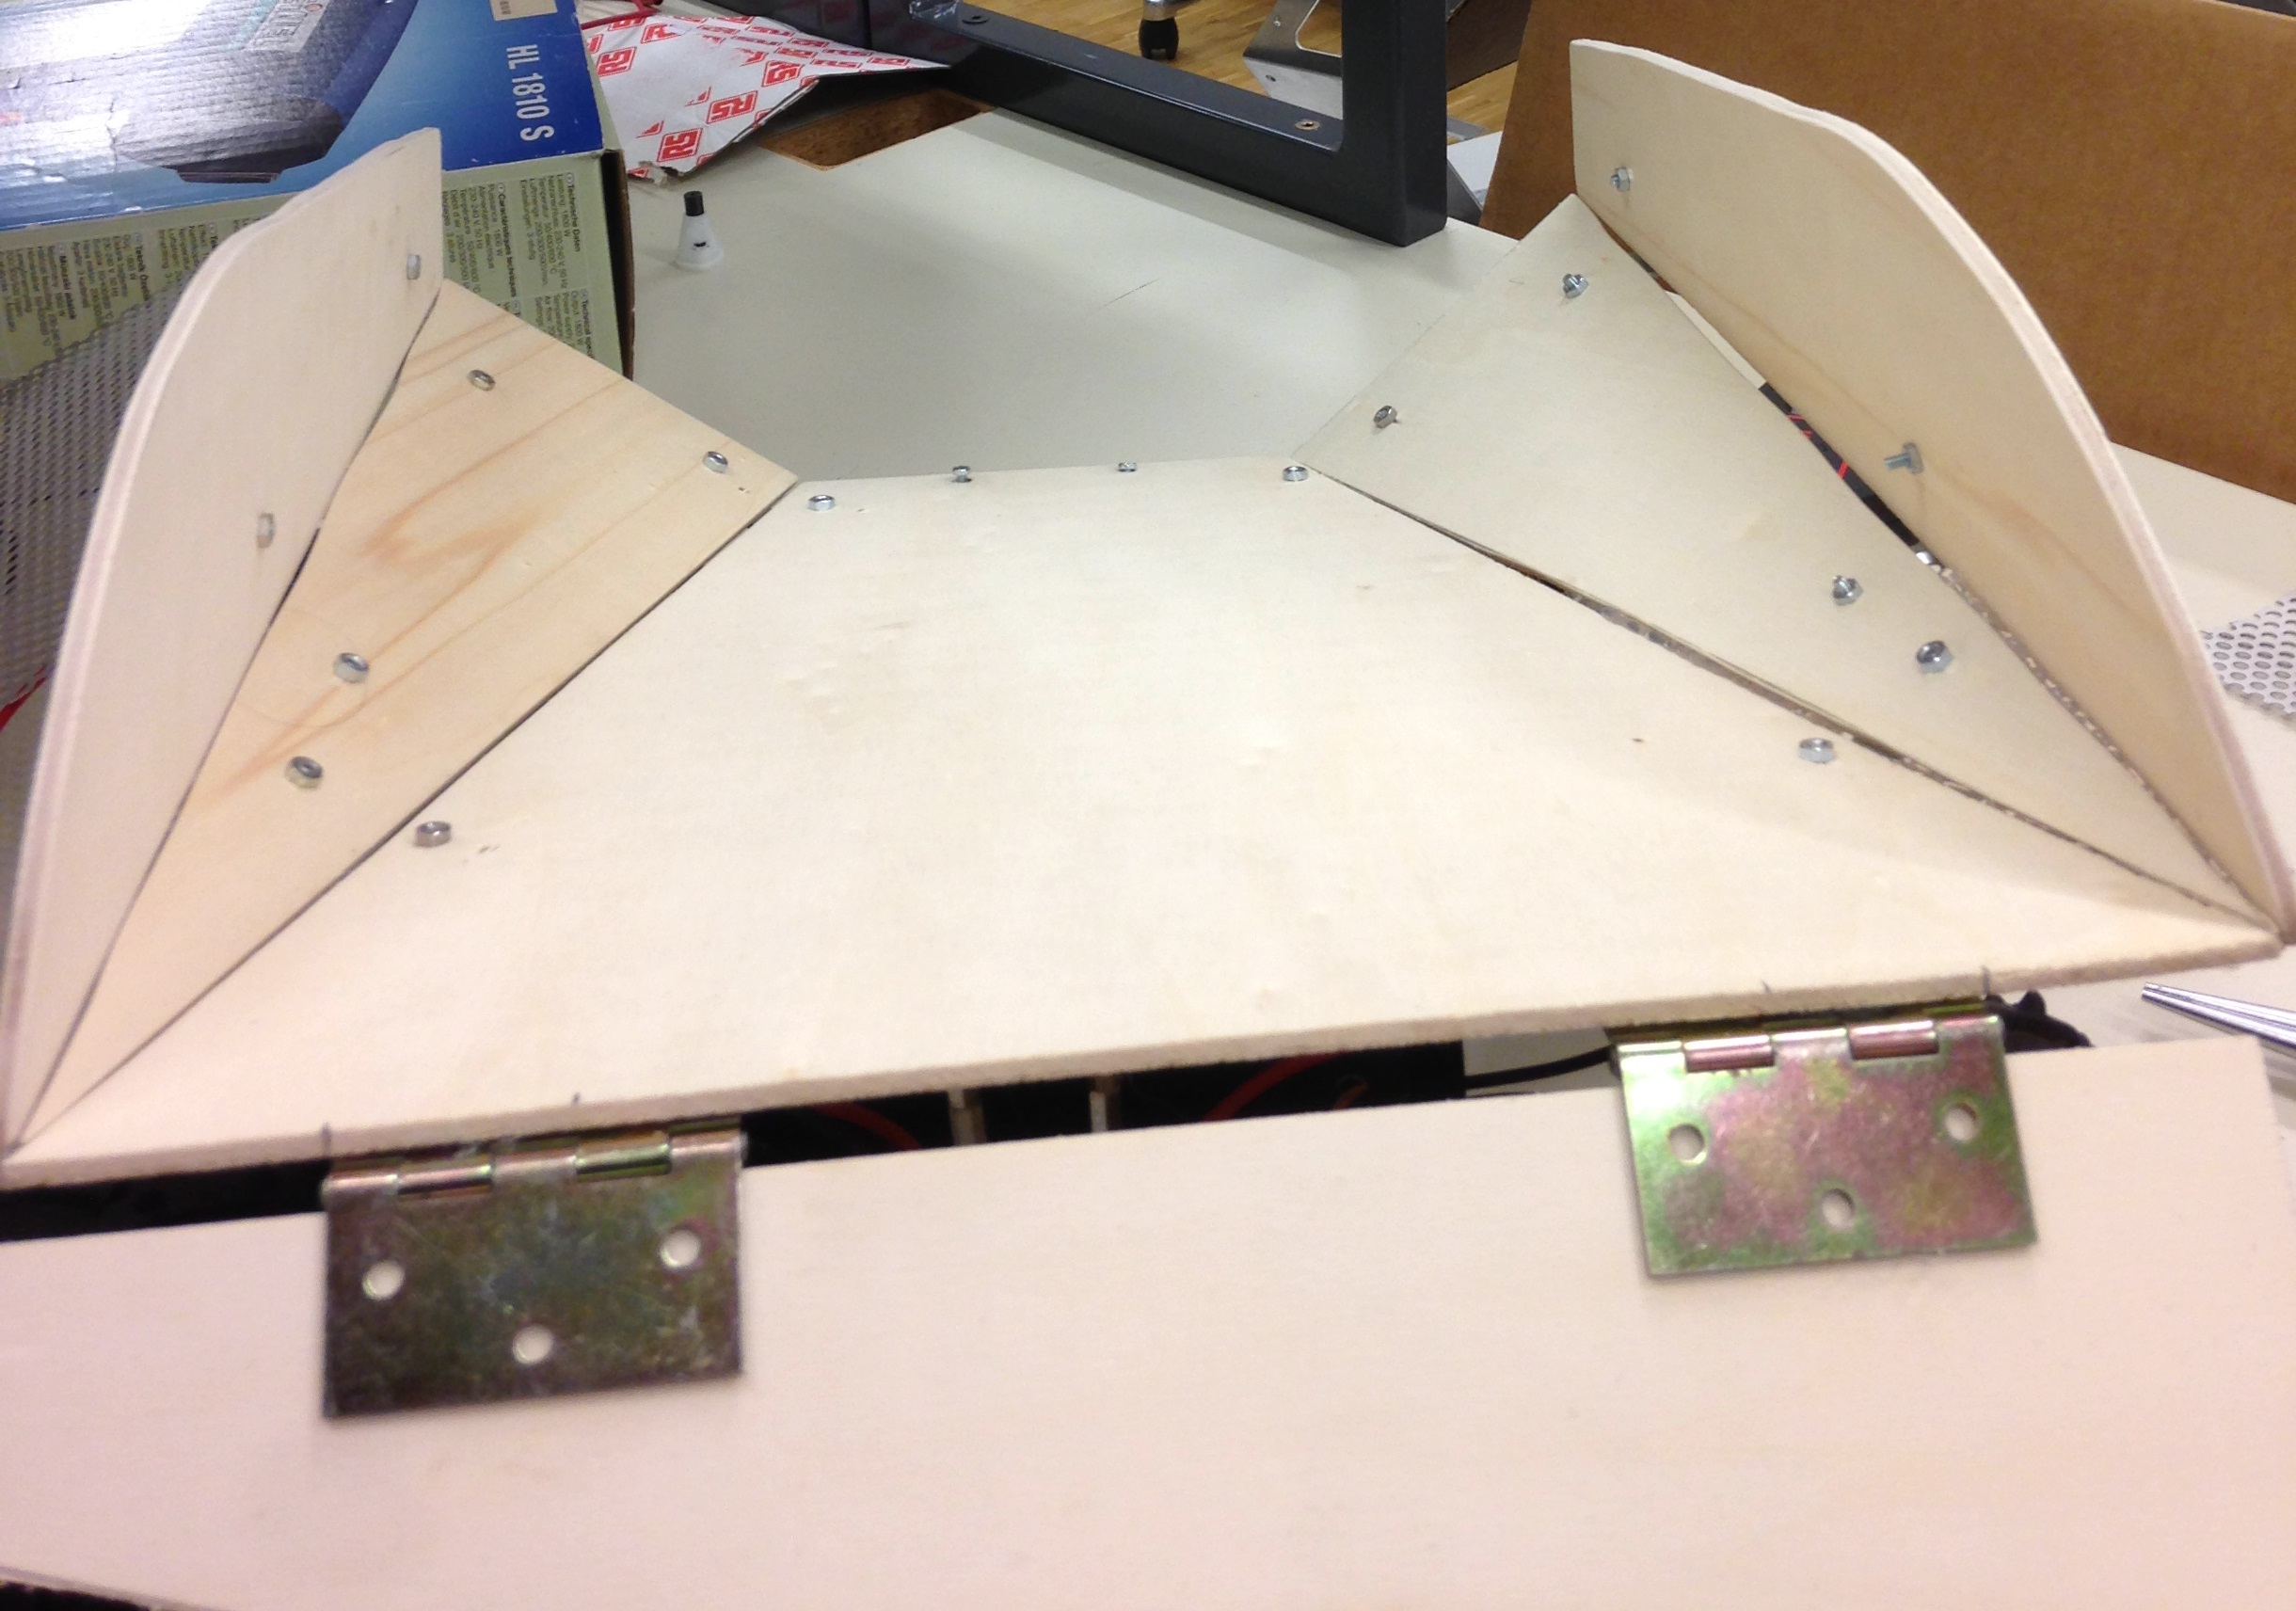
\includegraphics[width=0.3\textwidth]{WoodenModel3.JPG}
\end{center} 
 \caption{Upper-Front view of the robot's wooden model.}
\label{fig:WoodenModel3}
\end{wrapfigure}

Below the storage plate there is a hidden space that was decided to be reserved for the electronic components in order to guarantee a compact design where no space is wasted.
Thus all the electronics have been disposed under the storage part of the robot that is attached to the robot in a way to form a ramp in order to favorize the rolling of the bottles coming from the moving plate.
Moreover, this ramp was conceived in a way that it's height is adjustable, simplifying a lot the assembly of the final robot without incurring in unpredicted inaccuracies.
This adjustable slope mechanism is depicted by the Figure \ref{fig:AdjustableHeight3} below.

\begin{figure}[H]
 \centering
 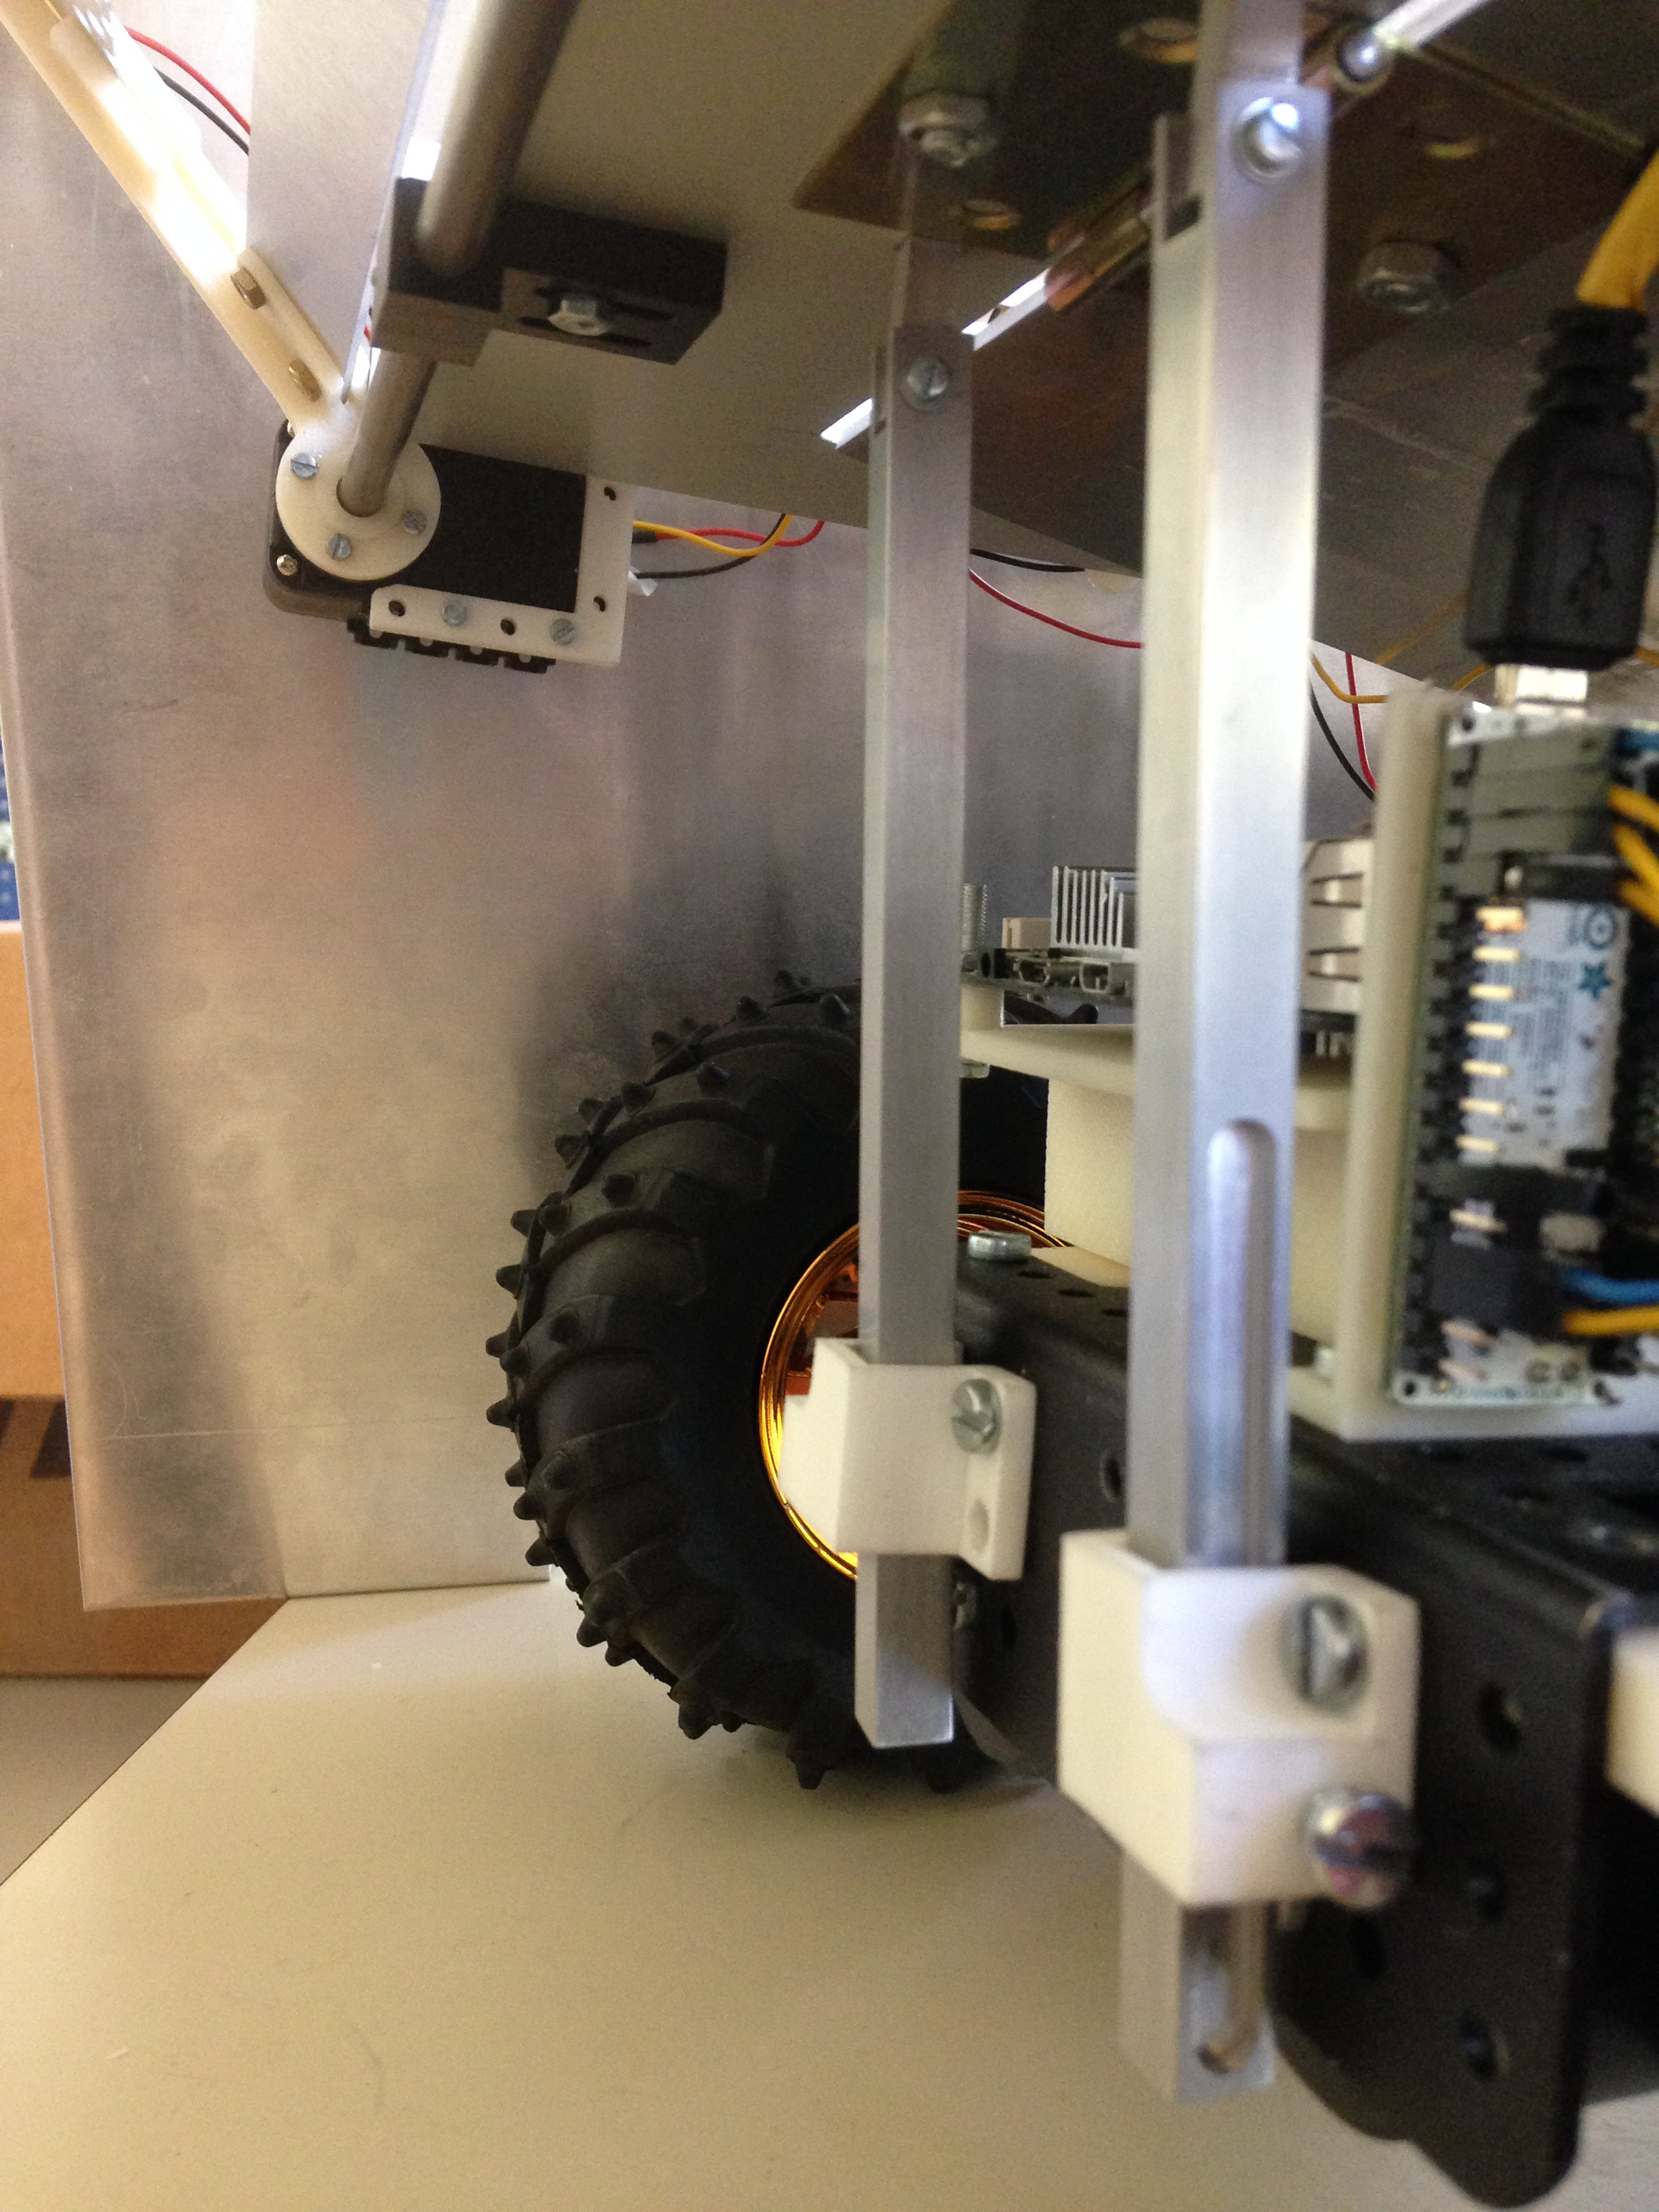
\includegraphics[width=0.5\textwidth]{AdjustableHeight3.JPG}
 \caption{Adjustable height mechanism of the storage compartement.}
\label{fig:AdjustableHeight3}
\end{figure}

After some test the slope for an aluminum plate that allowed the bottles to roll without getting stuck resulted to be of about $17^{\circ}$.
Furthermore, the electronics has been arranged in a way to allow an easy access to it and the batteries are accessible without needing the open the robot.

Thanks to the good quality of the described model manufactured in wood we have even been able to test the real actuators that afterwards have been used on the final model.
Being satisfied with this first mechanical verification of our idea a SolidWork model of the final robot has been realized.
This model is represented in figure \ref{fig:robotsdw}.

\begin{figure}[H]
 \centering
 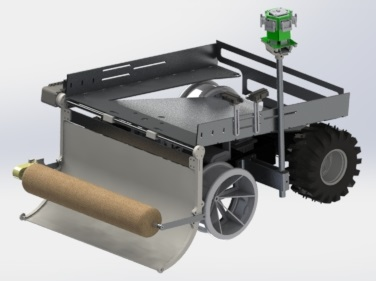
\includegraphics[width=0.8\textwidth]{robotsdw.JPG}
 \caption{Robot on solidworks.}
\label{fig:robotsdw}
\end{figure}

With only 15 manufactured parts, the robot's design was simple and it took less than a day to assemble. The top metal part is not present in the solidworks model, because it was not intended in the beginning. We found it among the remains of robots from previous years, and decided to recycle it on our own robot. 
Some parts were also modified compared to the original model, such as the lift, which was made larger to allow more bottles to be taken and in more possible orientations.  \\

After the approval of all the team members about the mechanical components that would have constituted the final robot, the mechanical 2D plans of all the single components have been produced to be then sent to the mechanical workshop and manufactured.
More complex parts have been printed with the further benefit of saving time by being able to be tested far earlier than the aluminum parts.
 In the meantime the “holders” of the sensors have been printed together with the electronic parts' boxes that have been conceived in order to guarantee their arrangement in the reserved space in the most proper way and allowing at the same time an easy access to them.
In the mechanical conception of the robot, great importance has been given to the design of the elevator shown in Figure \ref{fig:lift}.

\begin{figure}[H]
 \centering
 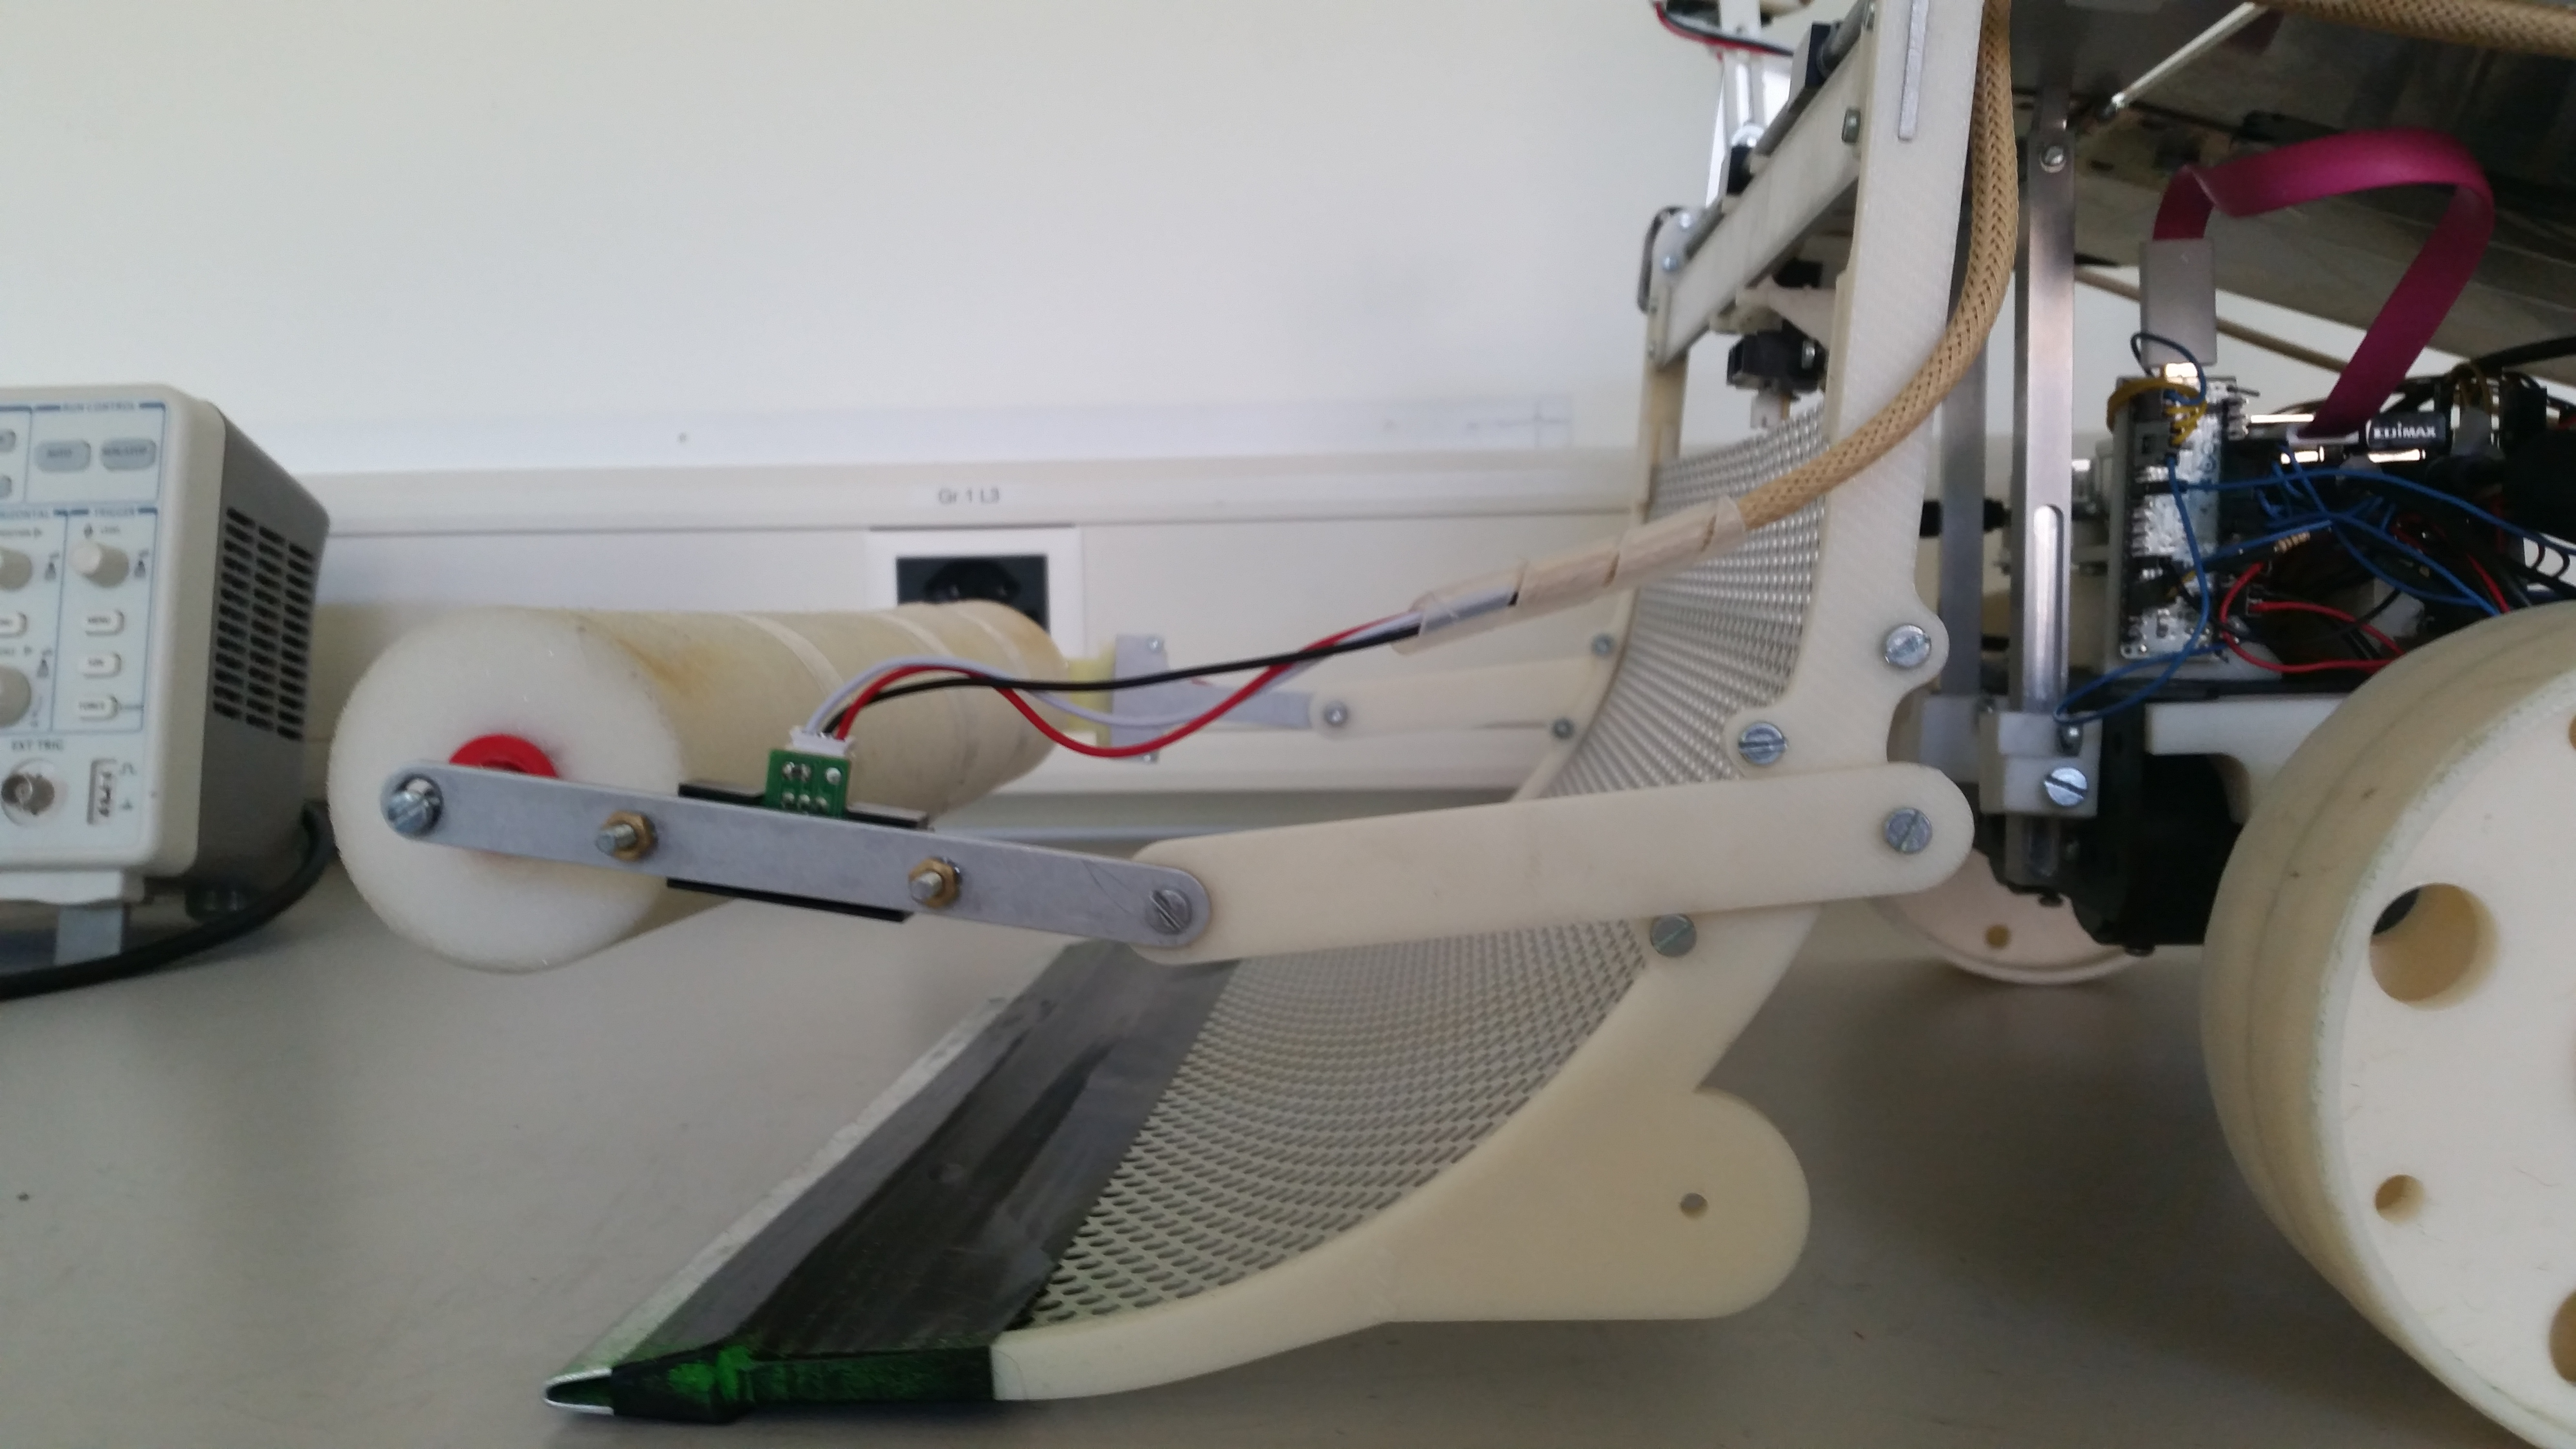
\includegraphics[width=0.5\textwidth]{lift.JPG}
 \caption{The robot's elevator.}
\label{fig:lift}
\end{figure}

With the design in Figure \ref{fig:lift}, the robot is able to pick up bottles in any position. See Figure \ref{fig:pickup} below.

\begin{minipage}{\linewidth}
      \centering
      \begin{minipage}{0.3\linewidth}
          \begin{figure}[H]
              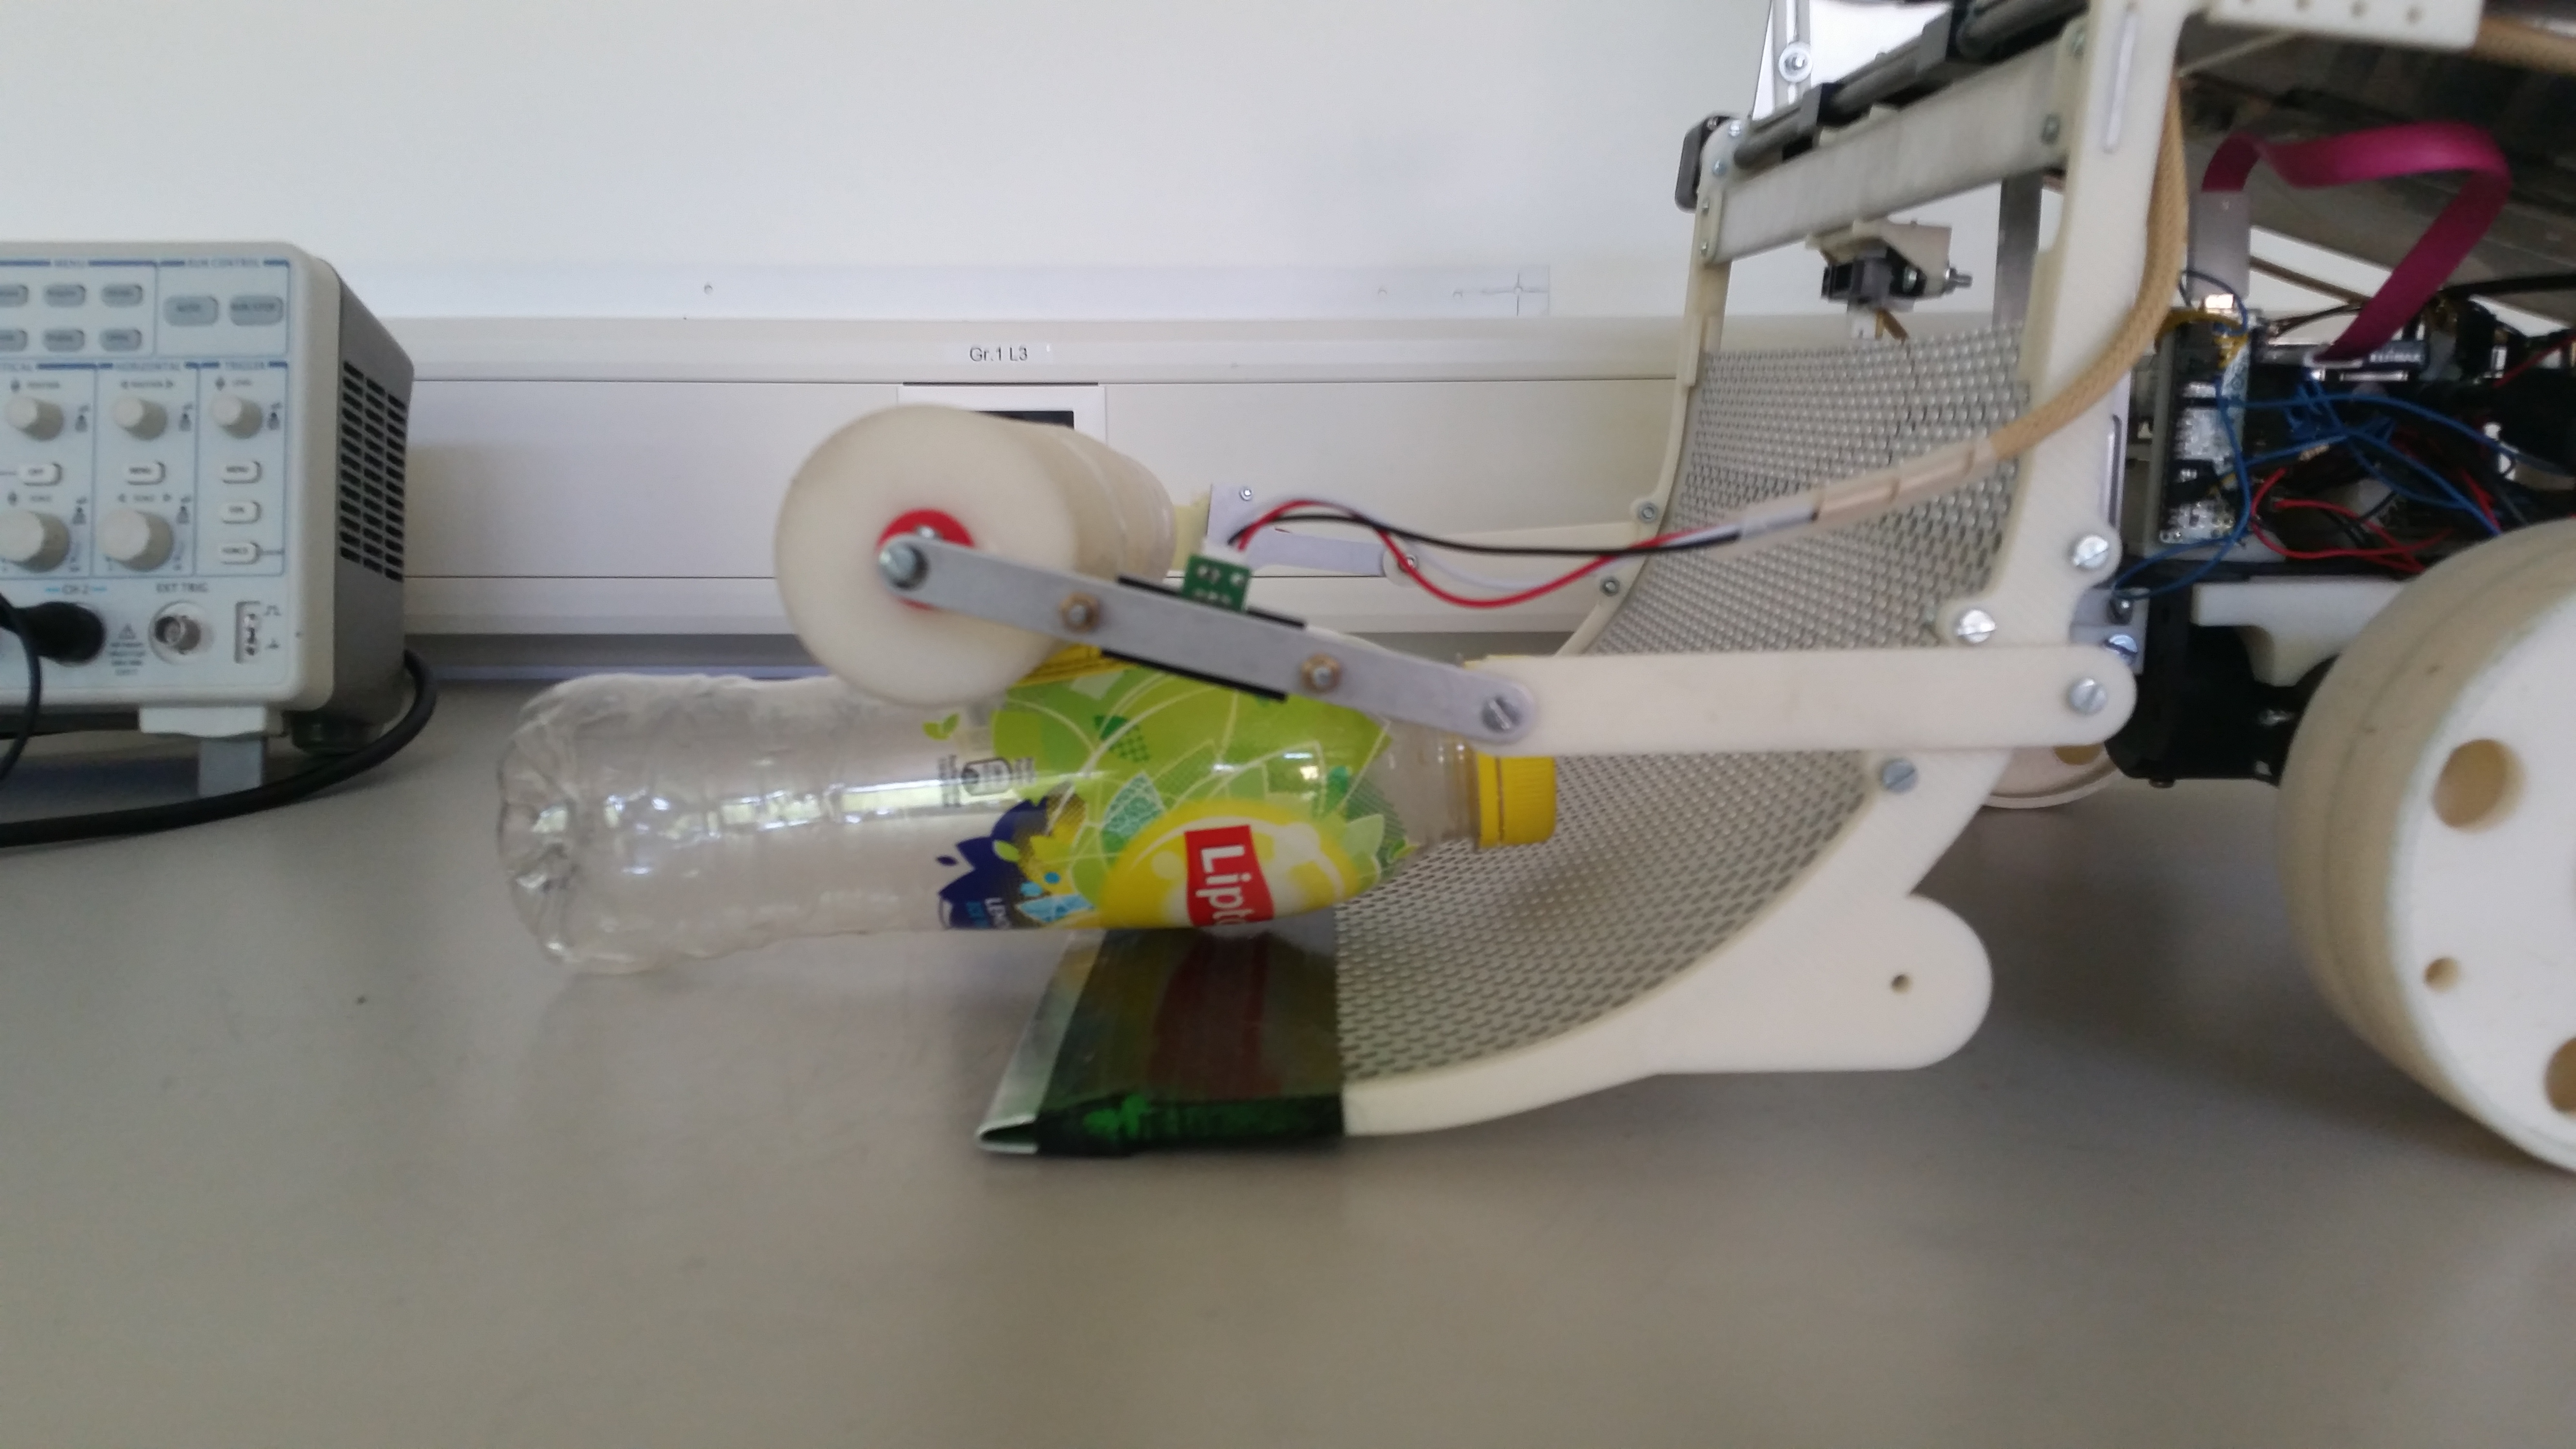
\includegraphics[width=\linewidth]{lift1.jpg}
              \caption{Bottle entering vertically.}
          \end{figure}
      \end{minipage}
      \hspace{0.05\linewidth}
      \begin{minipage}{0.3\linewidth}
          \begin{figure}[H]
              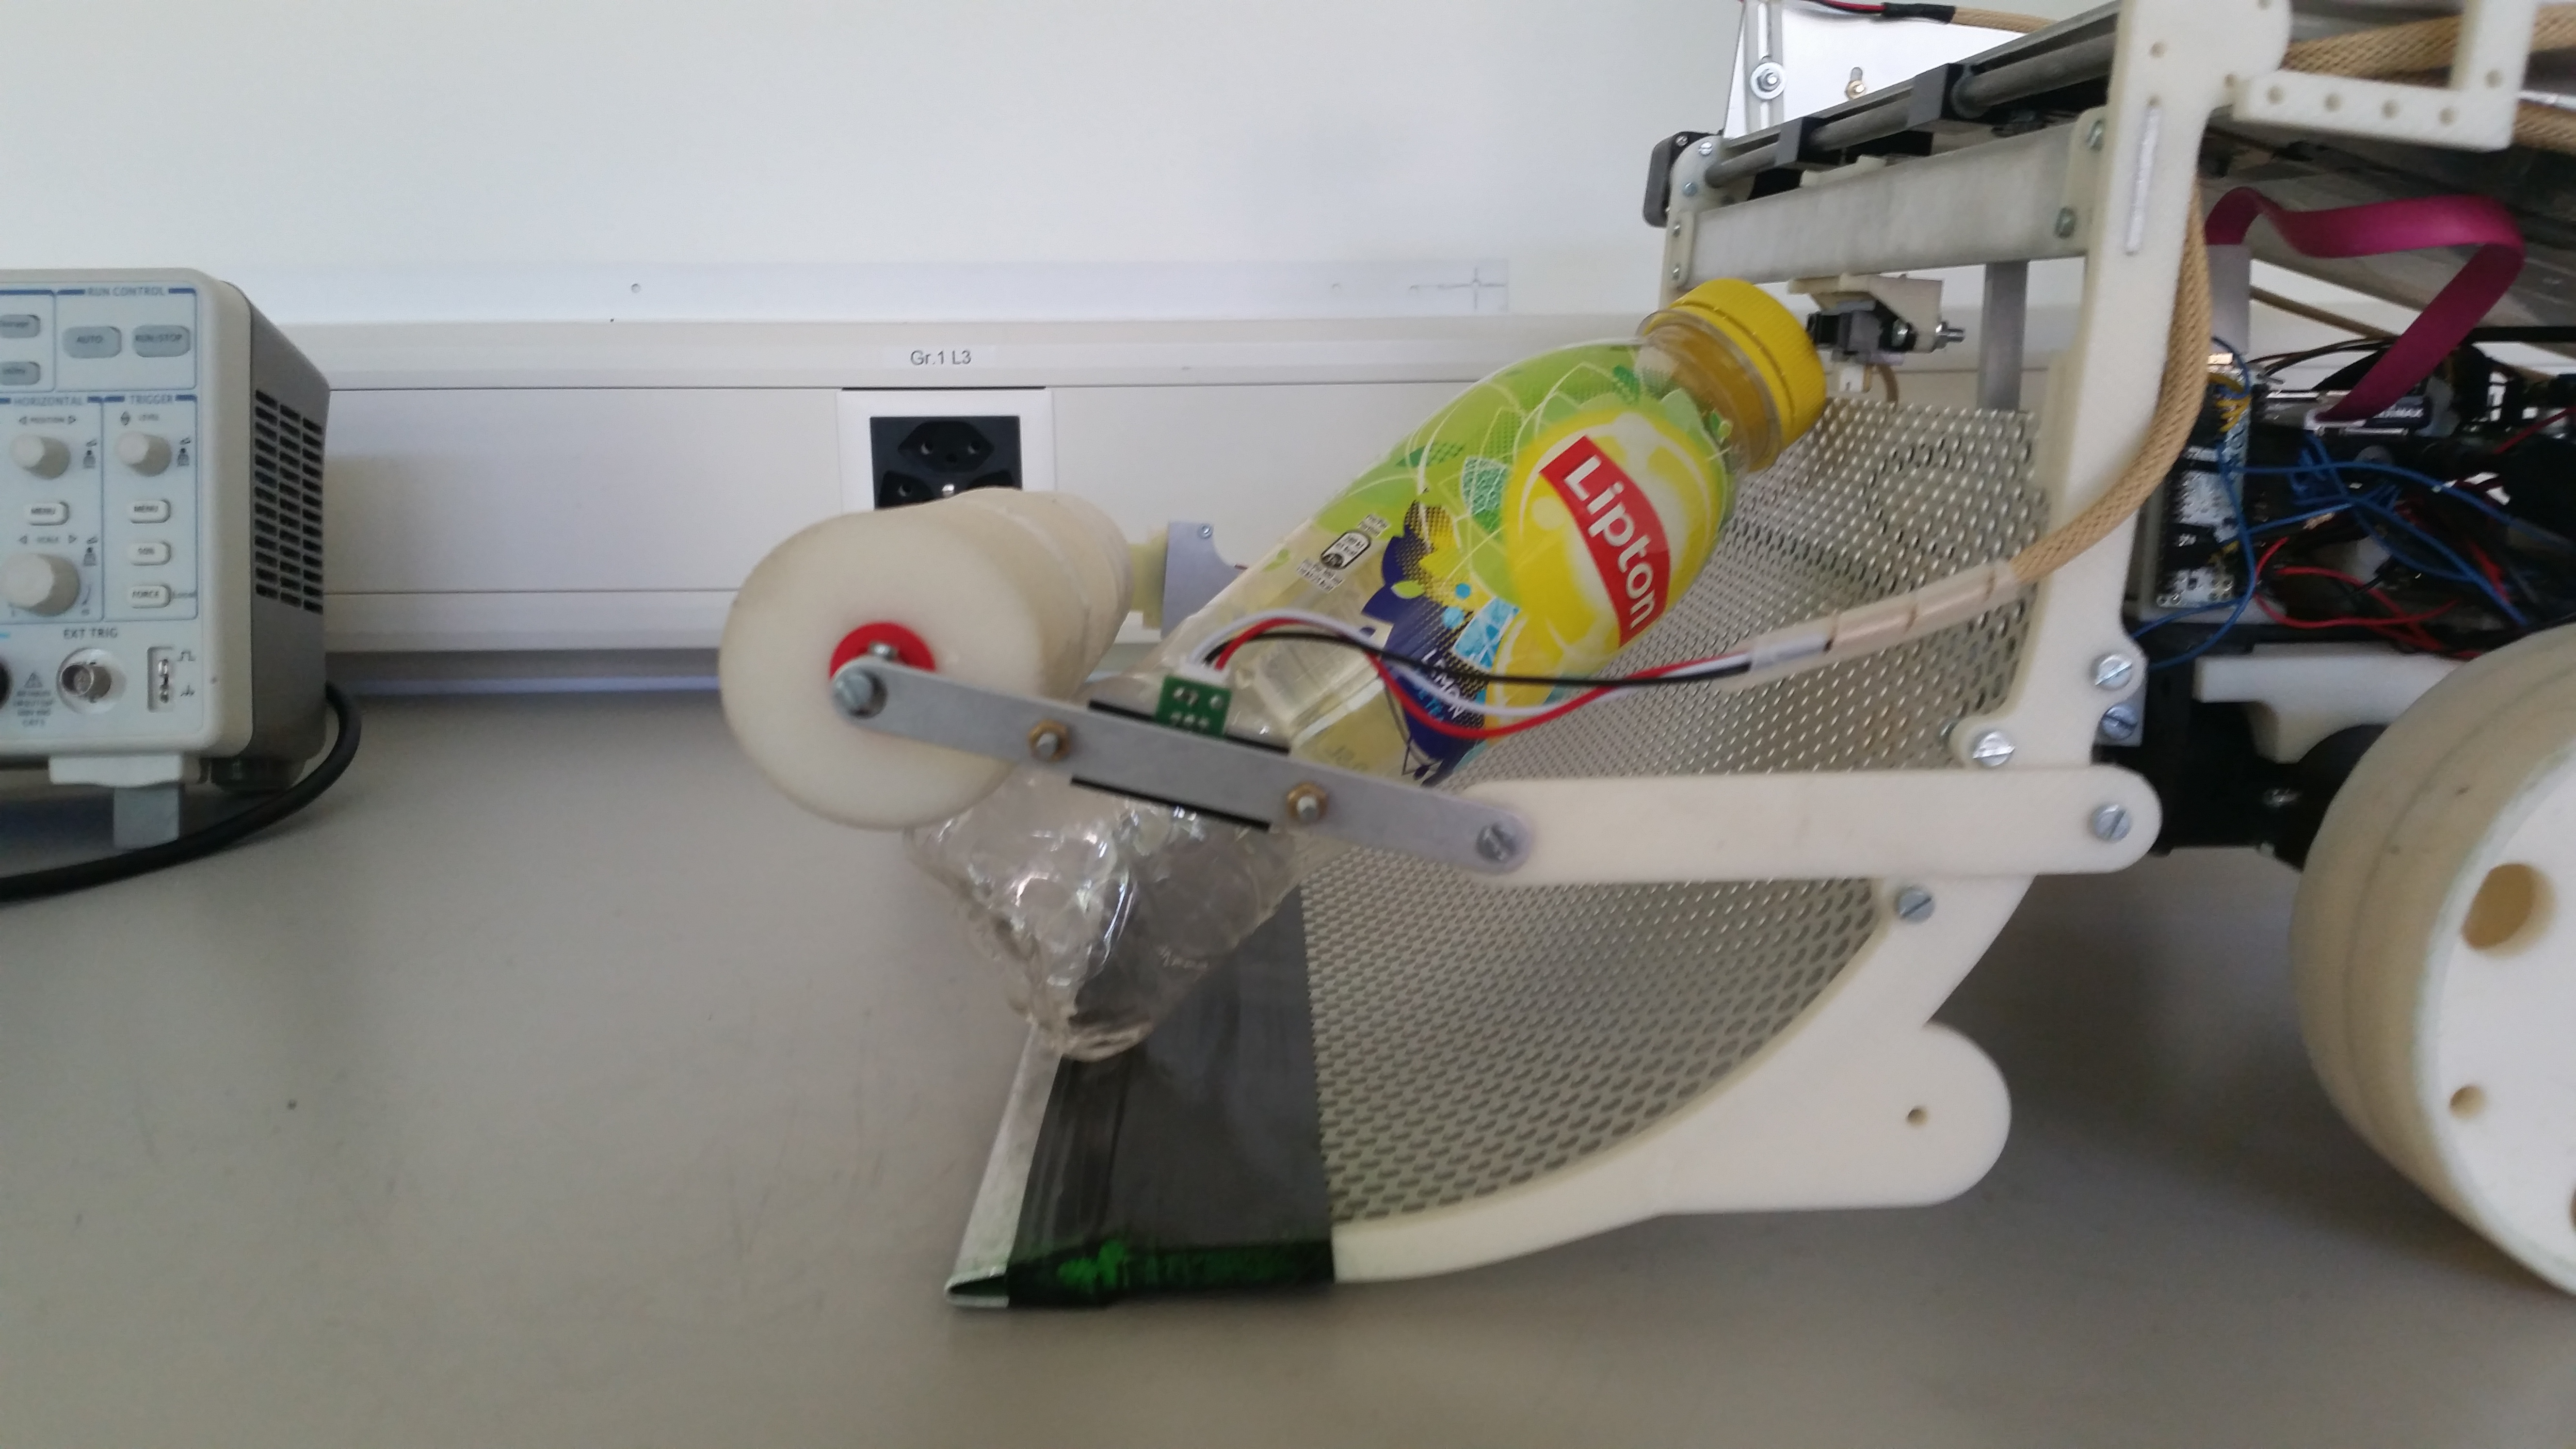
\includegraphics[width=\linewidth]{lift2.jpg}
              \caption{Bottle sliding up the ramp}
          \end{figure}
      \end{minipage}
      \hspace{0.05\linewidth}
      \begin{minipage}{0.3\linewidth}
          \begin{figure}[H]
              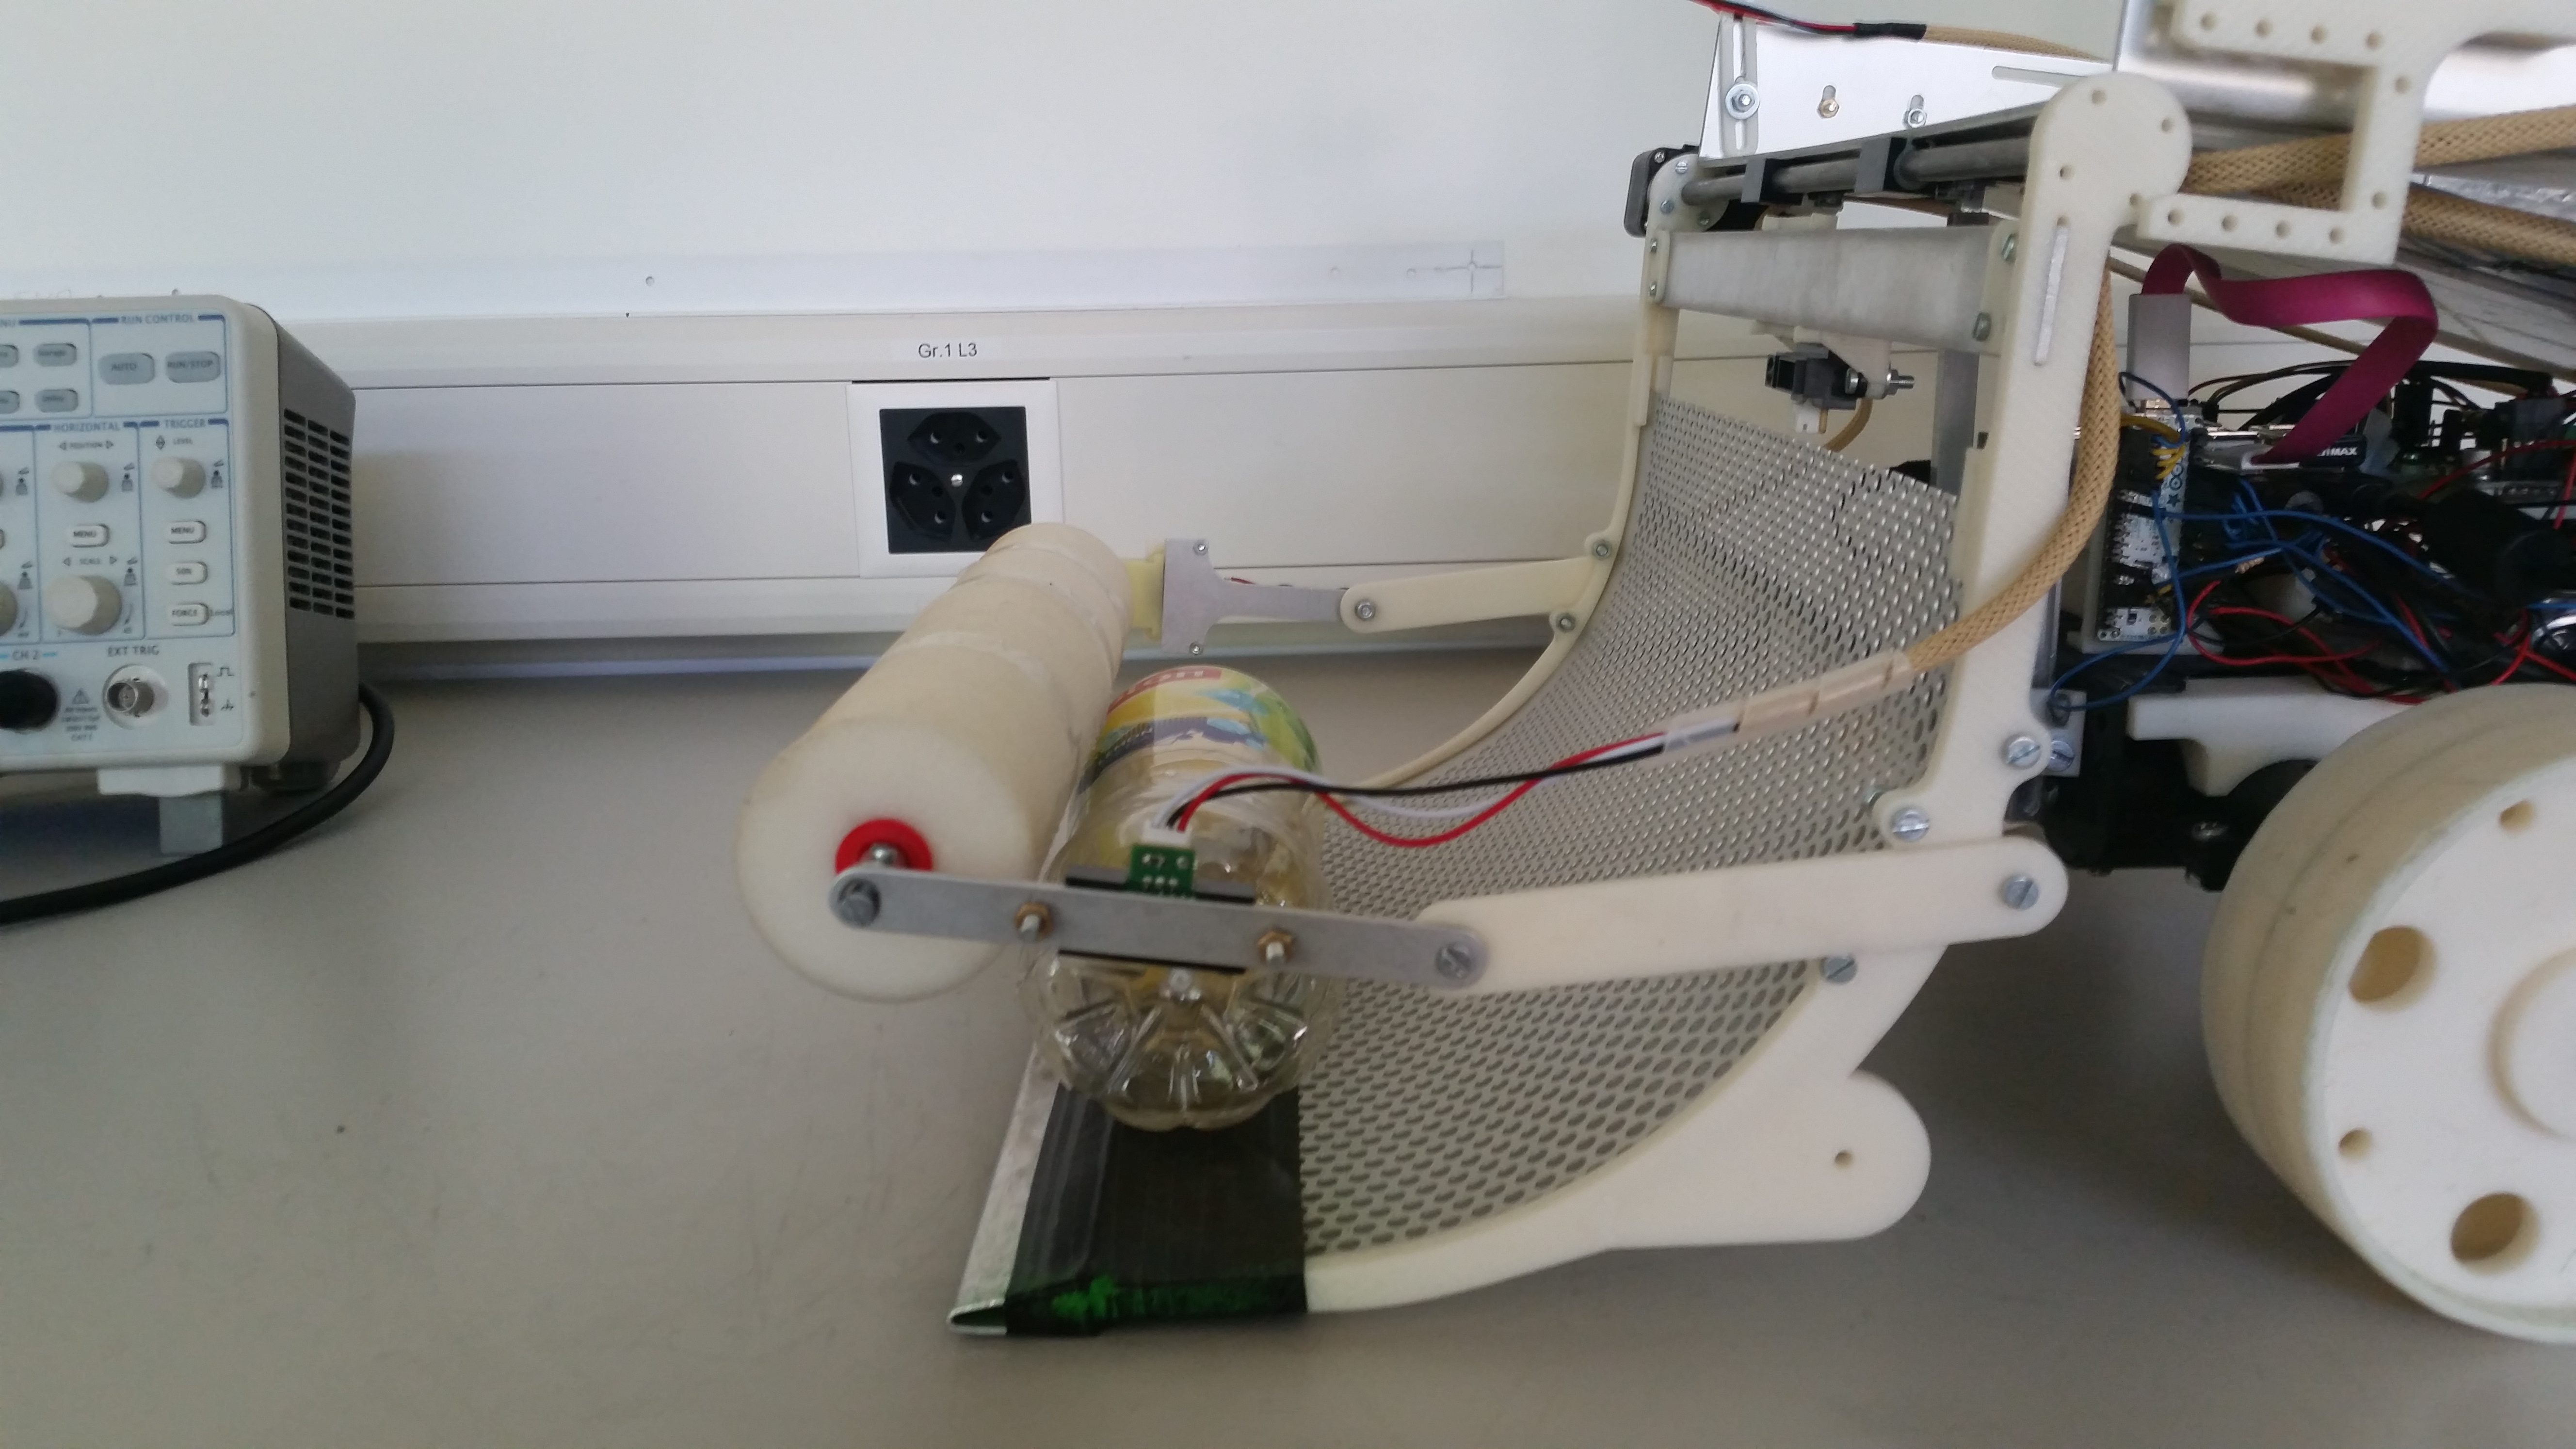
\includegraphics[width=\linewidth]{lift3.jpg}
              \caption{Bottle falling down on it's side.}
          \end{figure}
      \end{minipage}
      \label{fig:pickup}
  \end{minipage}

A lot of effort has been expended in order to make the electronic area, and in particular the zone reserved to batteries, easily accessible.
The storage compartment, can be detached in correspondance to the `adjustable height mechanism` and rotate around a pivoting system placed in correspondance to the end of the chassis.
The pivoting system is shown in Figure \ref{fig:PivotingSystem}.

\begin{figure}[H]
 \centering
 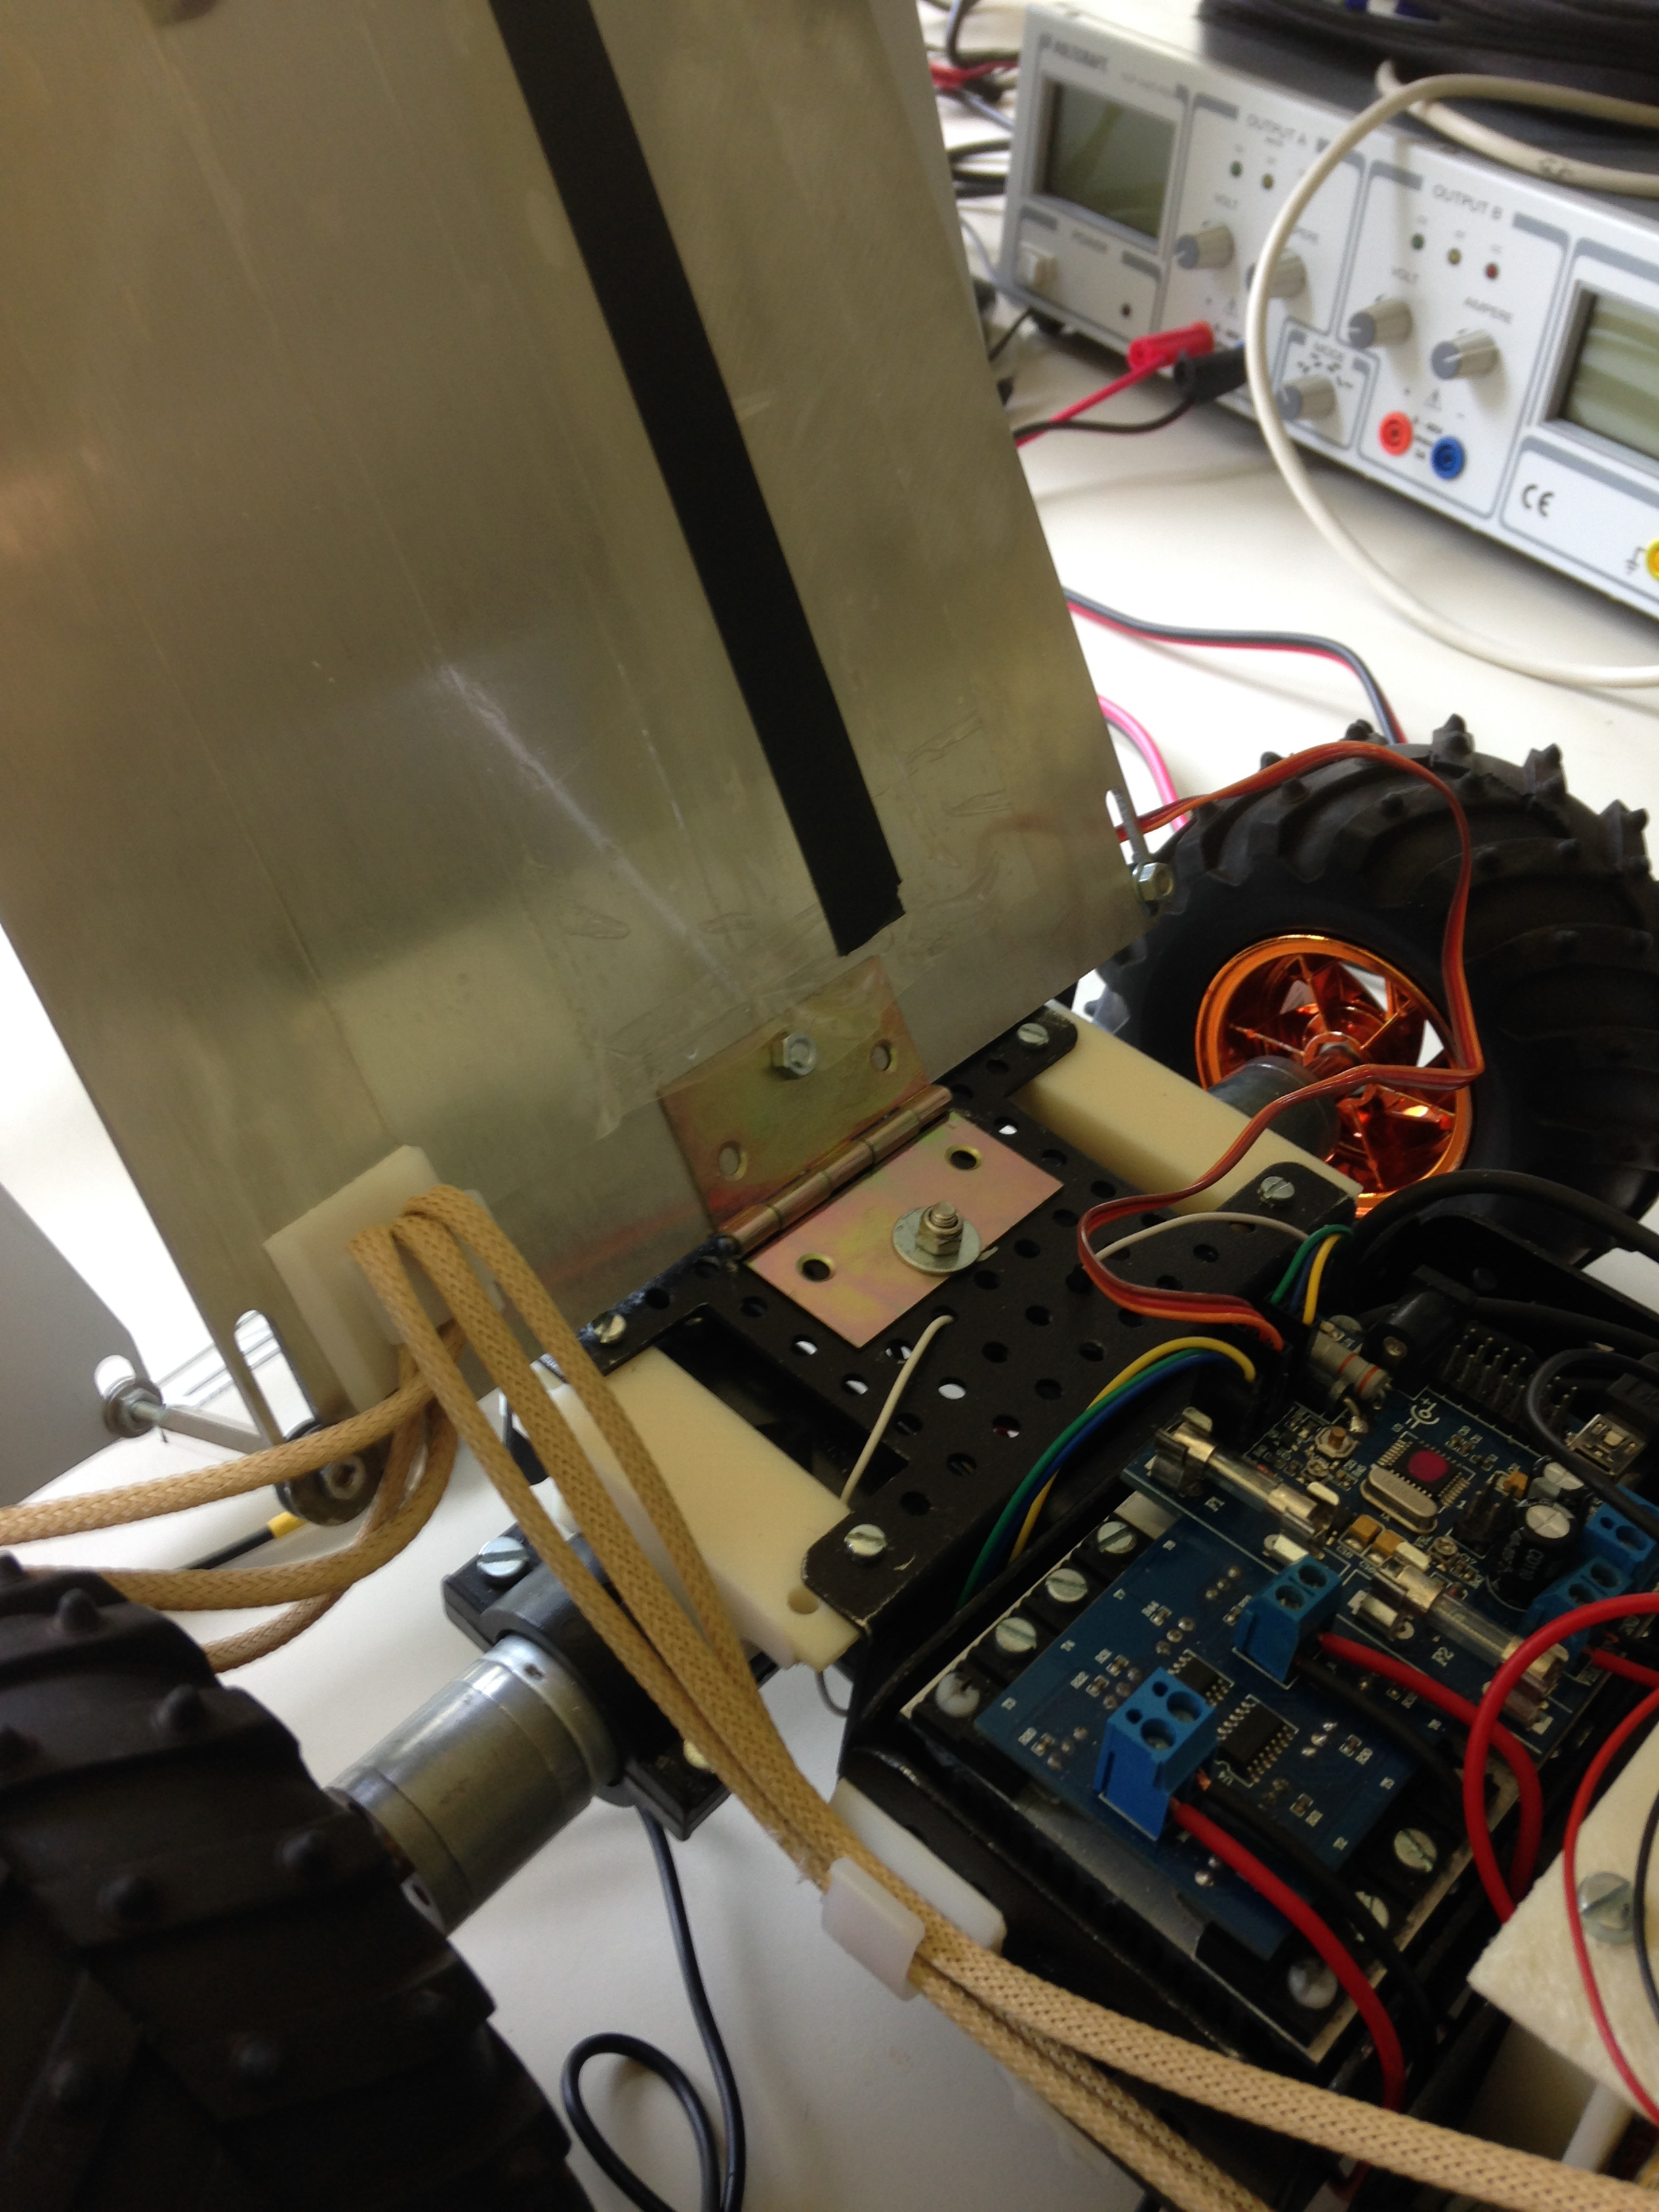
\includegraphics[width=0.3\textwidth]{PivotingSystem.JPG}
 \caption{Pivoting system for the storage ramp opening.}
\label{fig:PivotingSystem}
\end{figure}

This simple mechanism allows to access to the electronics that are arranged with the help of boxes which makes it possible to add and remove the batteries without having to remove any other component.

Another important feature, in terms of the mechanical conception of the robot, is the possibility to regulate the pointing direction of some sensors.
As it can be seen in Figure \ref{fig:PointingUS} and Figure \ref{fig:PointingCamera}, both the camera and the two front ultrasonic sensors are held by means of holders that allow to change the pointing direction.

\begin{figure}[H]
 \centering
 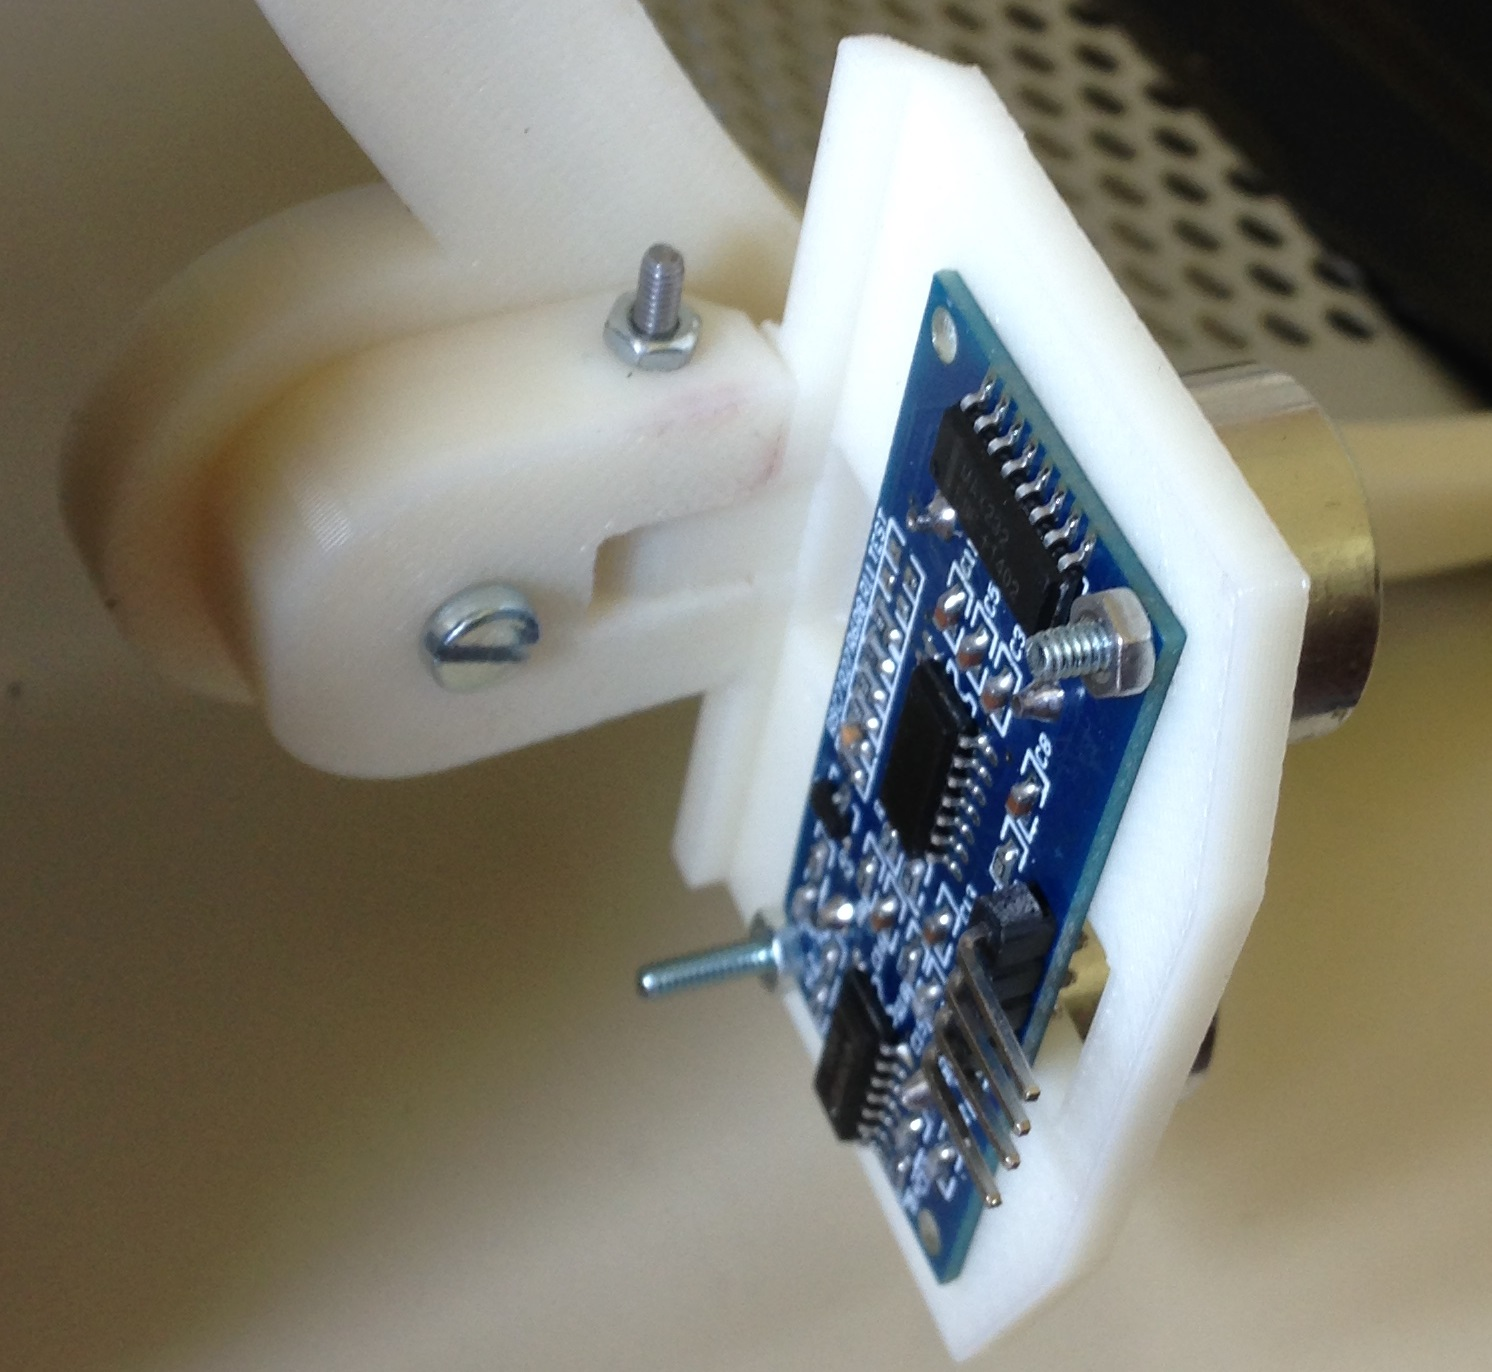
\includegraphics[width=0.3\textwidth]{PointingUS.JPG}
 \caption{Close view of the system that allows to rotate the Ultrasonic sensors.}
\label{fig:PointingUS}
\end{figure}

\begin{figure}[H]
 \centering
 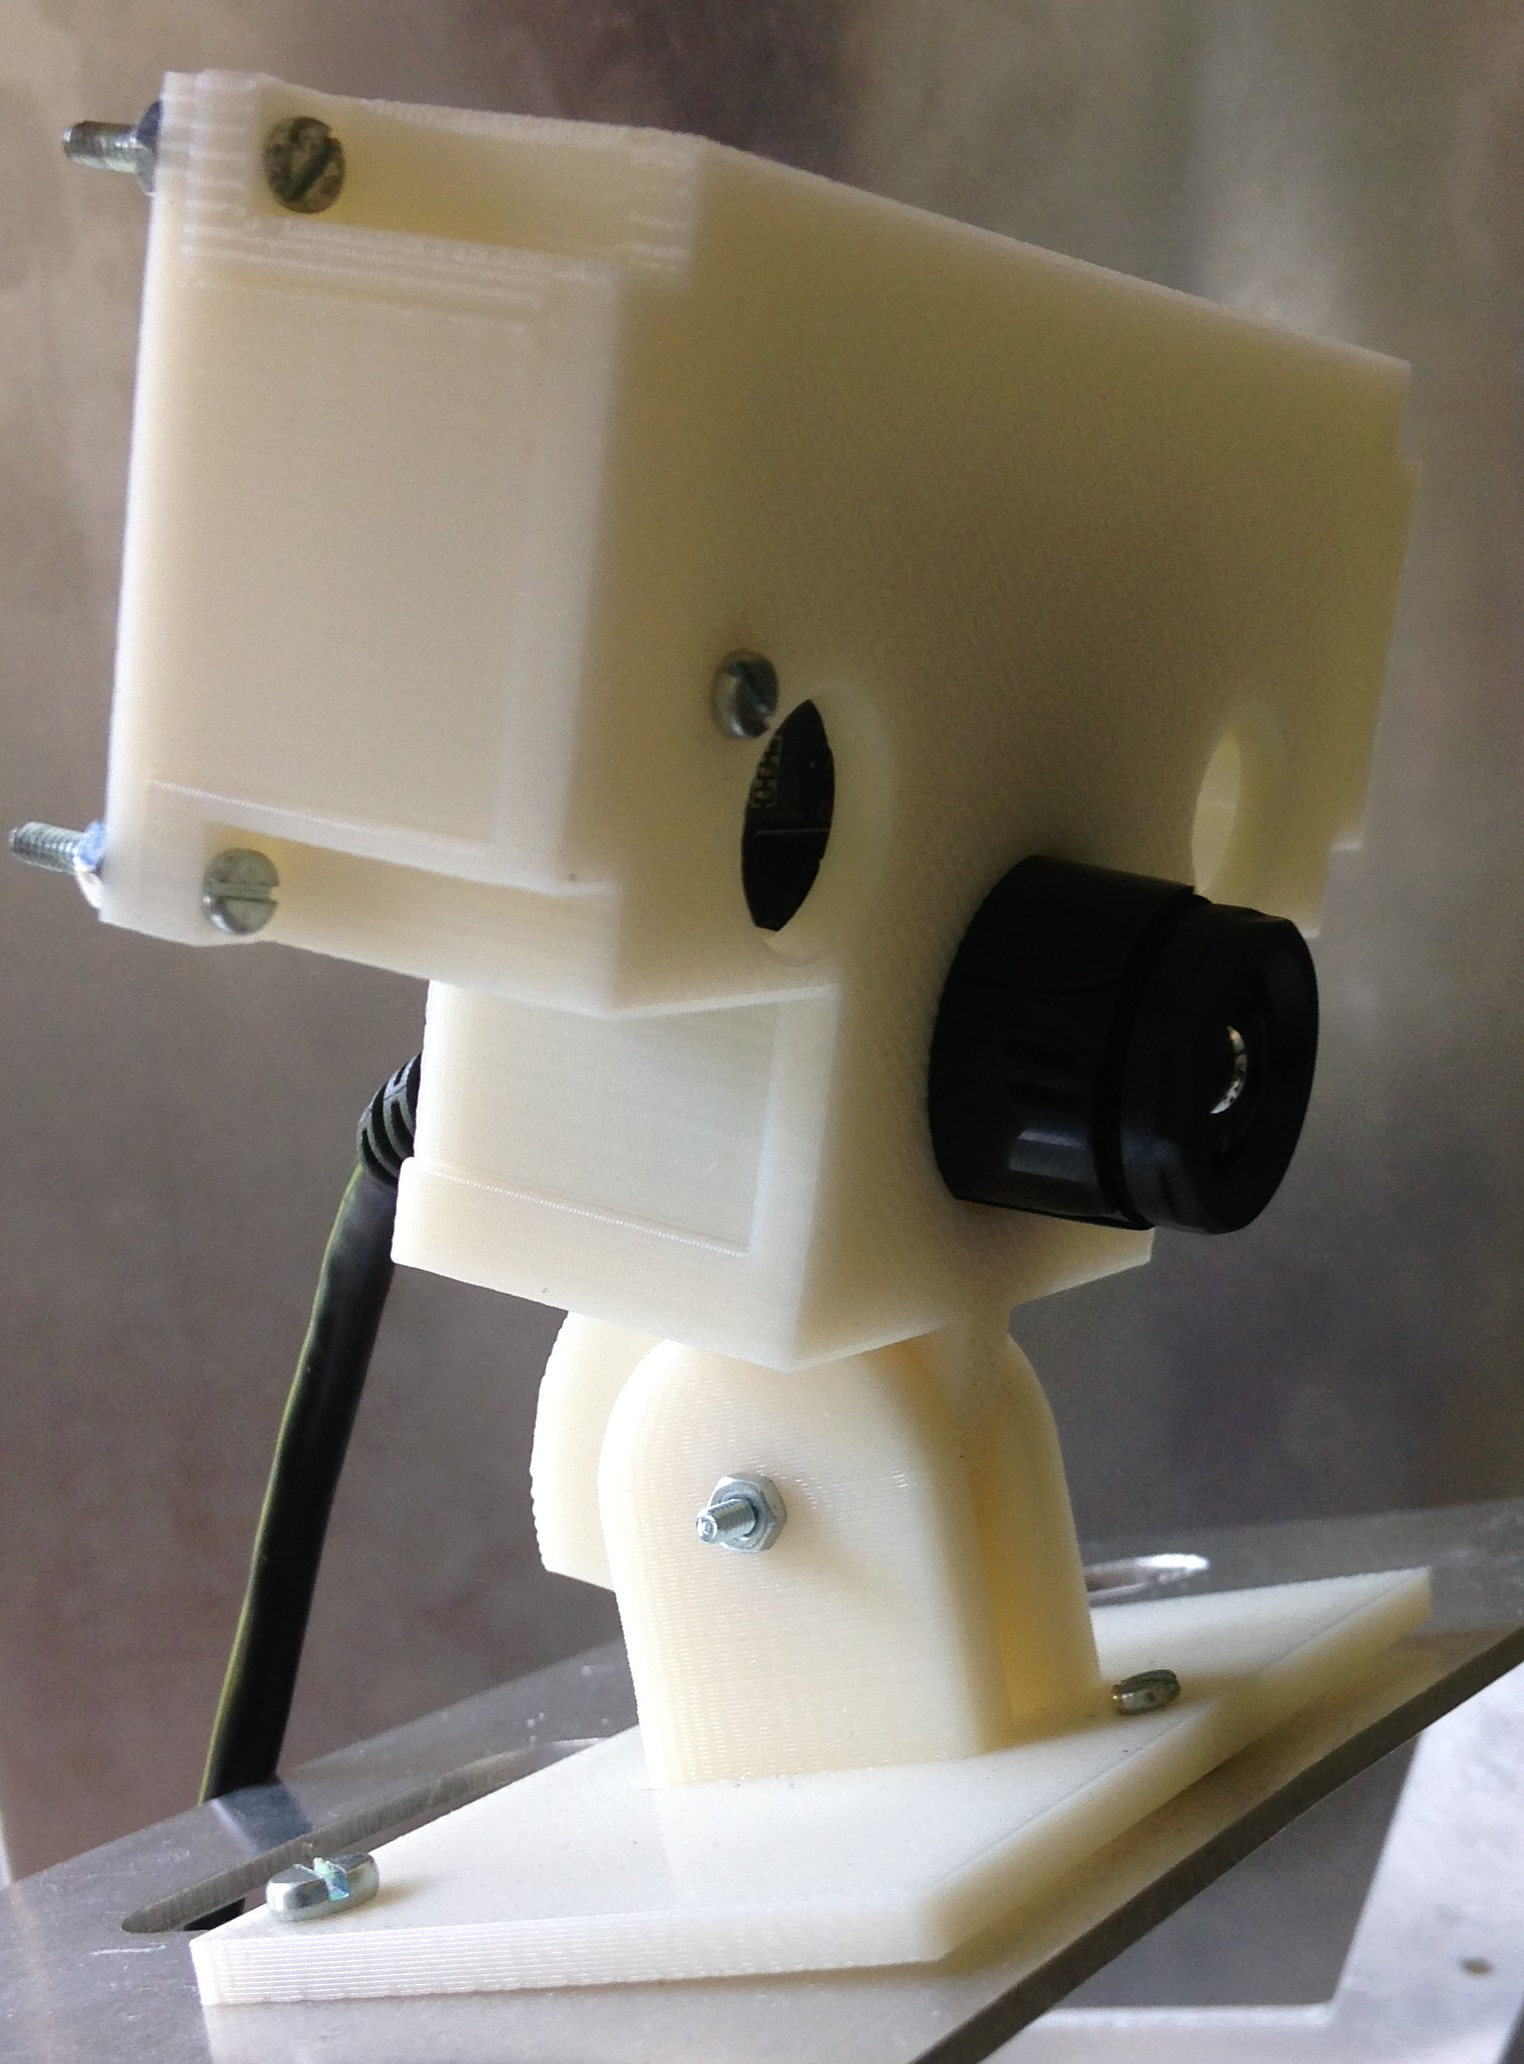
\includegraphics[width=0.3\textwidth]{PointingCamera.JPG}
 \caption{Close view of the system that allows to rotate the camera.}
\label{fig:PointingCamera}
\end{figure}

This was done since it was difficult to define an `a priori' for the sensors angles  that would return the best feedback in term of detection.
